% -------------------------------------------------------------------
\documentclass[usepdftitle=false,10pt]{beamer}

%encodings
\usepackage[utf8]{inputenc}
\usepackage[OT1]{fontenc}

%some useful packages
\usepackage[]{mathrsfs}
\usepackage[]{amssymb}
\usepackage[]{amsmath}
\usepackage[]{acronym}
\usepackage[]{listings}
\usepackage[]{xcolor}
\usepackage[]{graphicx}
\usepackage[]{textcomp} %for tilde


%\usepackage[english]{babel}
%\usepackage[utf8]{inputenc}
%\usepackage{amsmath}
%\usepackage{graphicx}
%\usepackage{amsfonts}
%\usepackage[]{xcolor}
%\usepackage[]{graphicx}
%\usepackage[]{textcomp} %for tilde

\hypersetup{pdftitle={ViennaCL}, pdfauthor={Florian Rudolf}}


%% Listings package START
\usepackage{color}
\usepackage{listings}

\definecolor{darkblue}{rgb}{0,0,.6}
\definecolor{darkred}{rgb}{.6,0,0}
\definecolor{darkgreen}{rgb}{0,.6,0}
\definecolor{red}{rgb}{.98,0,0}
\definecolor{lightgrey}{rgb}{0.98,0.98,0.98}


\lstloadlanguages{C++}
\lstset{%
  language=C++,
  basicstyle=\small\ttfamily,
  commentstyle=\itshape\color{darkgreen},
  keywordstyle=\bfseries\color{darkblue},
  stringstyle=\color{darkred},
  showspaces=false,
  showtabs=false,
  columns=fixed,
  backgroundcolor=\color{lightgrey},
  numbers=none,
  frame=single,
  numberstyle=\tiny,
  breaklines=true,
  showstringspaces=false,
  xleftmargin=0.1cm,
  escapechar=|
}%

\lstset{emphstyle=\color{red}}

%% Listings package STOP








\renewcommand{\matrix}[1]{\boldsymbol{#1}}
\renewcommand{\vector}[1]{\boldsymbol{#1}}
\renewcommand{\d}{\mathrm{d}}
\newcommand{\domelem}[1]{\boldsymbol{\mathrm{#1}}}
\newcommand{\kB}{k_\mathrm{B}}
\newcommand{\VT}{V_\mathrm{T}}
\newcommand{\q}{\mathrm{q}}
\newcommand{\LandauO}{\mathcal{O}}
\newcommand{\Bullet}{$\triangleright$}
\newcommand{\black}{ }
\newcommand{\ViennaCL}{\texttt{ViennaCL}}

\newcommand{\TODO}[1]{{\color{red}\textbf{TODO: #1}}}

%\setlength{\fboxrule}{1pt}

%\renewcommand{\seriesdefault}{\bfdefault}
%\usepackage{helvet}

\graphicspath{{figures/}}           % in which folder all the figures are
\newcommand{\tn}   {\textnormal}

%\mode<presentation>

%\usetheme{Boadilla}
%\usecolortheme{albatross}
%\setbeamercolor{normal text}{bg=blue}
%\setbeamercolor{title}{fg=white}
%\setbeamercolor{structure}{fg=white}
%\setbeamertemplate{headline}
%{\begin{beamercolorbox}[left,sep=.3cm]{title in head/foot} \LARGE\insertsection \end{beamercolorbox}}
%\setbeamerfont{title}{size=\Large} % Der Titel auf der Titlepage
%\setbeamerfont{footline}{size=\scriptsize}
% Disable Navigation symbols:
%\setbeamertemplate{navigation symbols}{}

% table of contents, depth
\setcounter{tocdepth}{2}

% modify at will
\setbeamercovered{transparent}

\usetheme[height=0.3cm,width=0.8cm,shadow=false]{iue}


\author[Florian Rudolf]{Florian Rudolf}
%\author[Karl Rupp]{Karl Rupp}
%\author[Josef Weinbub]{Josef Weinbub}

\institute[TU Wien]
{ \footnotesize
  Institute for Microelectronics \\
  Institute for Analysis and Scientific Computing \\
  [1em]
  Technische Universit\"at Wien, Austria  
}

\title[ViennaCL]{  
\includegraphics[width=0.5\textwidth]{figs/viennacl-logo.pdf} \\ \\ The Vienna Computing Library \\ }
%\titlegraphic{
% \fcolorbox{black}{white}{ \hspace{1cm}
%    
\includegraphics[keepaspectratio=true,height=1.5cm]{TUVienna.pdf} \hspace{2cm}
%    
\includegraphics[keepaspectratio=true,height=1.5cm]{logo_asc.pdf} \hspace{2cm} 
%    \includegraphics[keepaspectratio=true,height=1.5cm]{logo_iue.pdf} \hspace{1cm}
%   }
%}
\date[CG Libs - Smart Libraries for Computer Graphics 2013]{ \footnotesize CG Libs - Smart Libraries for Computer Graphics 2013}

\setbeamertemplate{blocks}[default]
%\setbeamercolor{block title}{bg=}
\setbeamercolor{block body}{bg=}

\begin{document}
\newenvironment{equationfett}{\Large\begin{equation}}{\end{equation} \normalsize}
\newenvironment{boldalign}{\Large\begin{align*}}{\end{align*} \normalsize}
% -------------------------------------------------------------070605
% Dokumentbeginn 
% -------------------------------------------------------------------
\begin{frame}[plain]
 \frametitle{~}
 \titlepage
\end{frame}



\begin{frame}{Talk Overview}

  \begin{block}{Session 1}
    \begin{itemize}
    \item Introduction to ViennaCL
    \item How-To: ViennaCL Basics
    \end{itemize}
  \end{block}
  
  \begin{block}{Session 2}
    \begin{itemize}
    \item How-To: Advanced ViennaCL
    \item ViennaCL: Behind the curtain
    \end{itemize}
  \end{block}

\end{frame}



% ViennaCL Introduction


%%%%%%%%%%%%%%%%%%%%%%%%%%%%%%%%%%% Introduction to ViennaCL %%%%%%%%%%%%%%%%%%%%%%%%%%%%%%%%%%%%


\begin{frame}{ }
 \begin{center}
  \Large \textbf{Introduction to \ViennaCL}
 \end{center}
\end{frame}


\begin{frame}{Introduction to \ViennaCL}

\begin{block}{What to expect}
  \begin{itemize}
   \item What is ViennaCL
   \item OpenCL
   \item History of ViennaCL
   \item Goals of ViennaCL
   \item Installation of ViennaCL
  \end{itemize}
\end{block}

\end{frame}




\begin{frame}{What Is \ViennaCL?}

\begin{block}{What is it about the Name?}
\begin{itemize}
  \item The beautiful city of \textbf{Vienna}
  \item Open\textbf{CL}
\end{itemize}
\end{block}

\vspace{3.4cm}

\end{frame}


% \begin{frame}{What Is \ViennaCL?}
% 
% \begin{block}{What is it about the Name?}
% \begin{itemize}
%   \item The beautiful city of \textbf{Vienna}
%   \item Open\textbf{CL}
% \end{itemize}
% \end{block}
% 
% {
% \centering
% 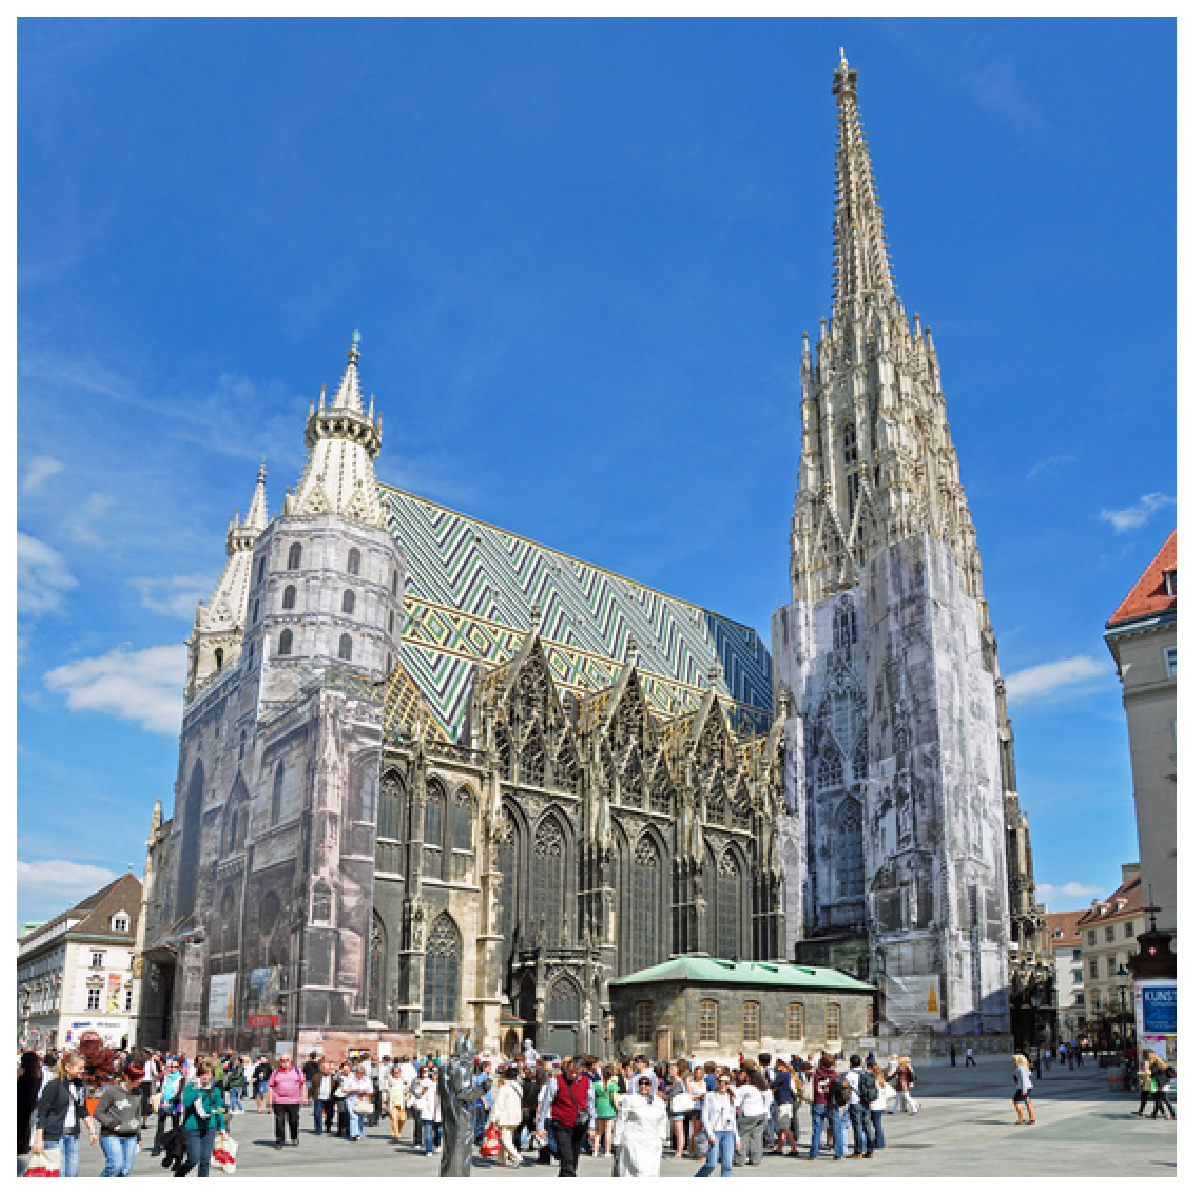
\includegraphics[width=0.3\textwidth]{figs/vienna.eps}
% }
% 
% \end{frame}


% \begin{frame}{What Is \ViennaCL?}
% 
% \begin{block}{What is it about the Name?}
% \begin{itemize}
%   \item The beautiful city of \textbf{Vienna}
%   \item Open\textbf{CL}
% \end{itemize}
% \end{block}
% 
% {
% \centering
% 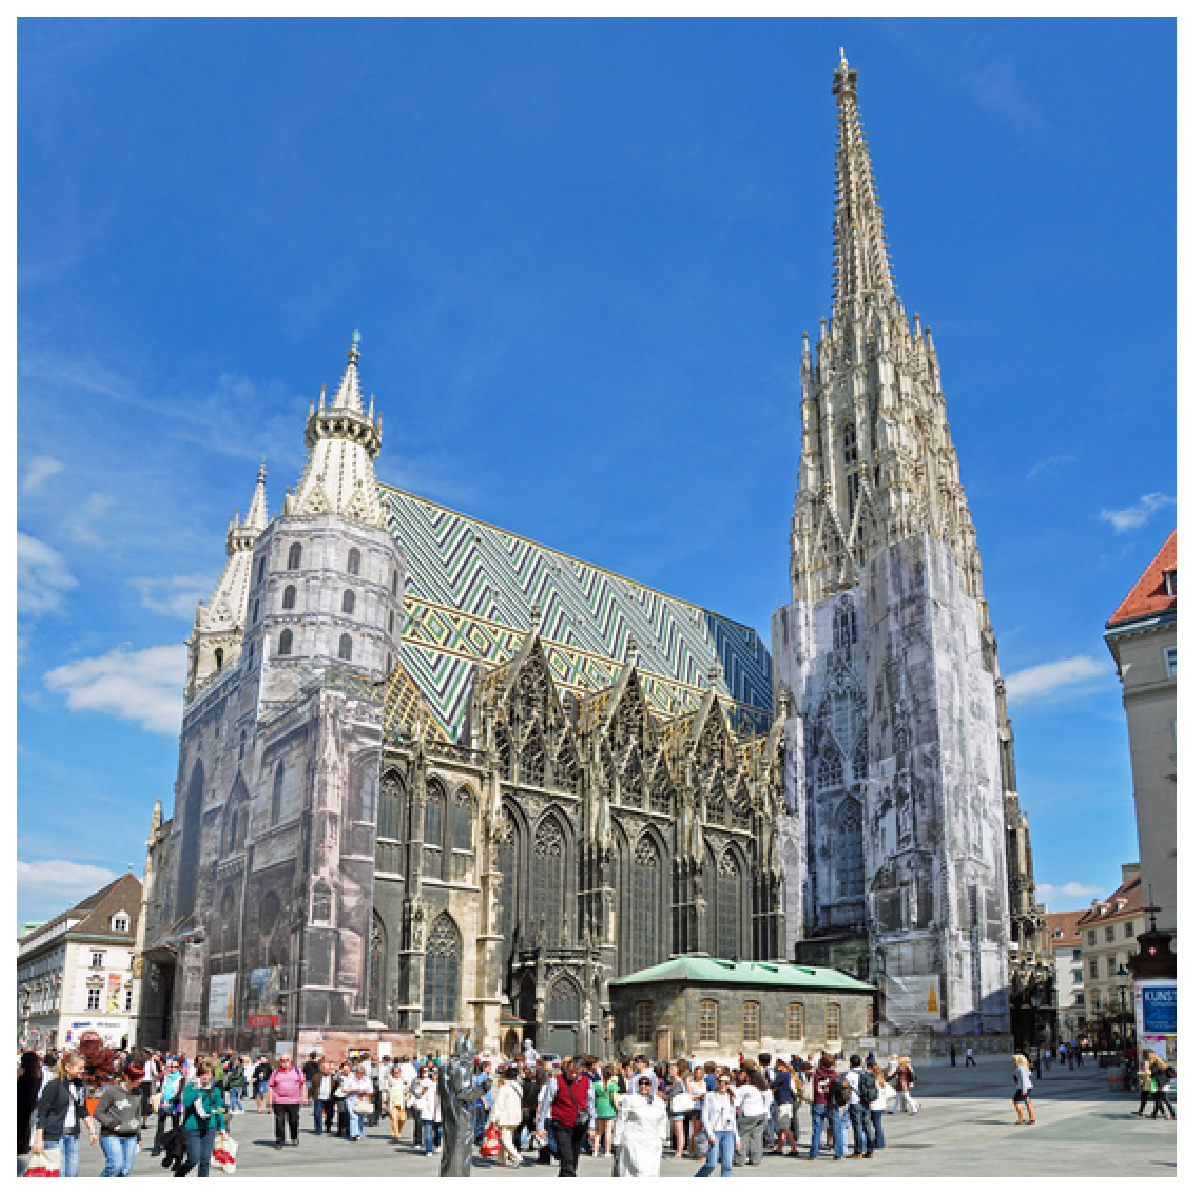
\includegraphics[width=0.3\textwidth]{figs/vienna.eps}
% \hspace{2cm}
% 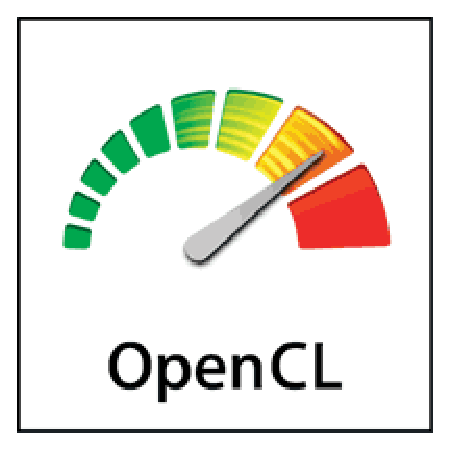
\includegraphics[width=0.3\textwidth]{figs/opencl_logo.eps}
% }
% 
% \end{frame}





\begin{frame}{History of OpenCL}

\begin{minipage}{0.6\textwidth}
\begin{block}{Prior to 2008}
  \begin{itemize}
   \item OpenCL developed by Apple Inc.
  \end{itemize}
\end{block}
\end{minipage} \hfill
\begin{minipage}{0.2\textwidth}
 
\includegraphics[width=0.99\textwidth]{figs/opencl.jpg}
\end{minipage}


\begin{block}{2008}
  \begin{itemize}
   \item OpenCL working group formed at Khronos Group
   \item OpenCL specification 1.0 released
  \end{itemize}
\end{block}

\begin{block}{2010}
  \begin{itemize}
   \item OpenCL 1.1 (multi-device, subbuffer manipulation)
  \end{itemize}
\end{block}

\begin{block}{2011}
  \begin{itemize}
   \item OpenCL 1.2 (device partitioning)
  \end{itemize}
\end{block}

\end{frame}

%%%%%%%%%%%%%%%%%%%%%%% Device %%%%%%%%%%%%%%%%%%%%%%


% \begin{frame}{OpenCL Platform Model}
%  \begin{center}
%    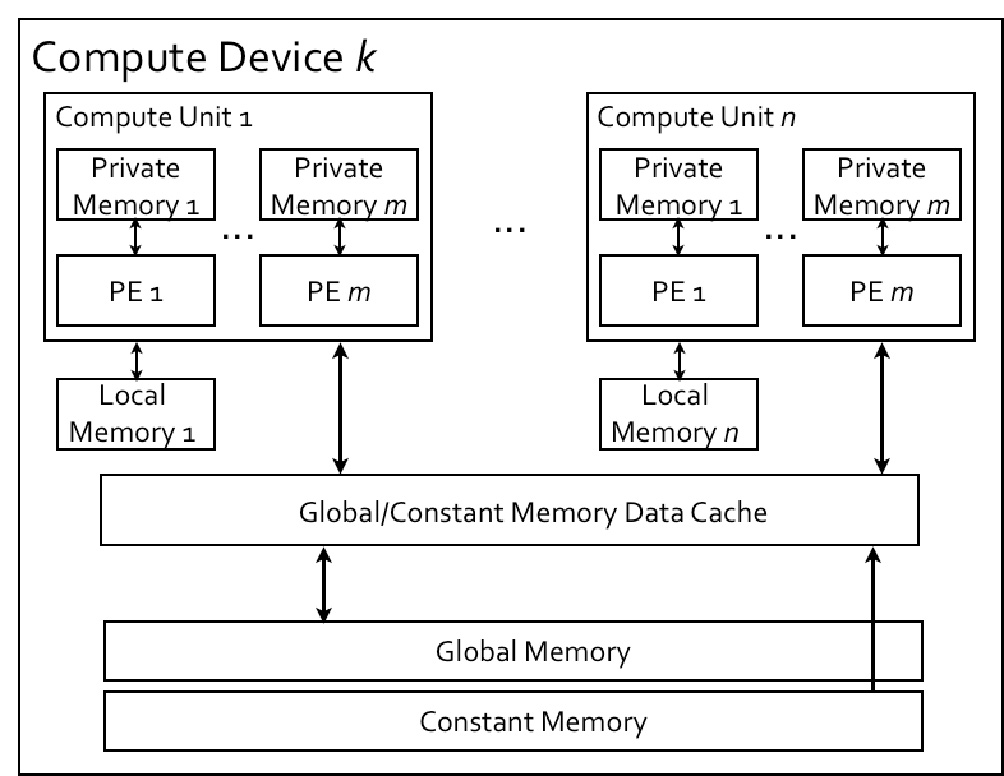
\includegraphics[width=0.8\textwidth]{figs/opencl-device.jpg} \\
%  \end{center}
%   {\tiny http://developer.amd.com/documentation/articles/PublishingImages/opencl\_figure5.jpg}
%   \vspace{0.5cm}
% \end{frame}


%%%%%%%%%%%%%%%%%%%% Platform Model %%%%%%%%%%%%%%%%%%%%%%

\begin{frame}{OpenCL Platform Model}
 \begin{center}
   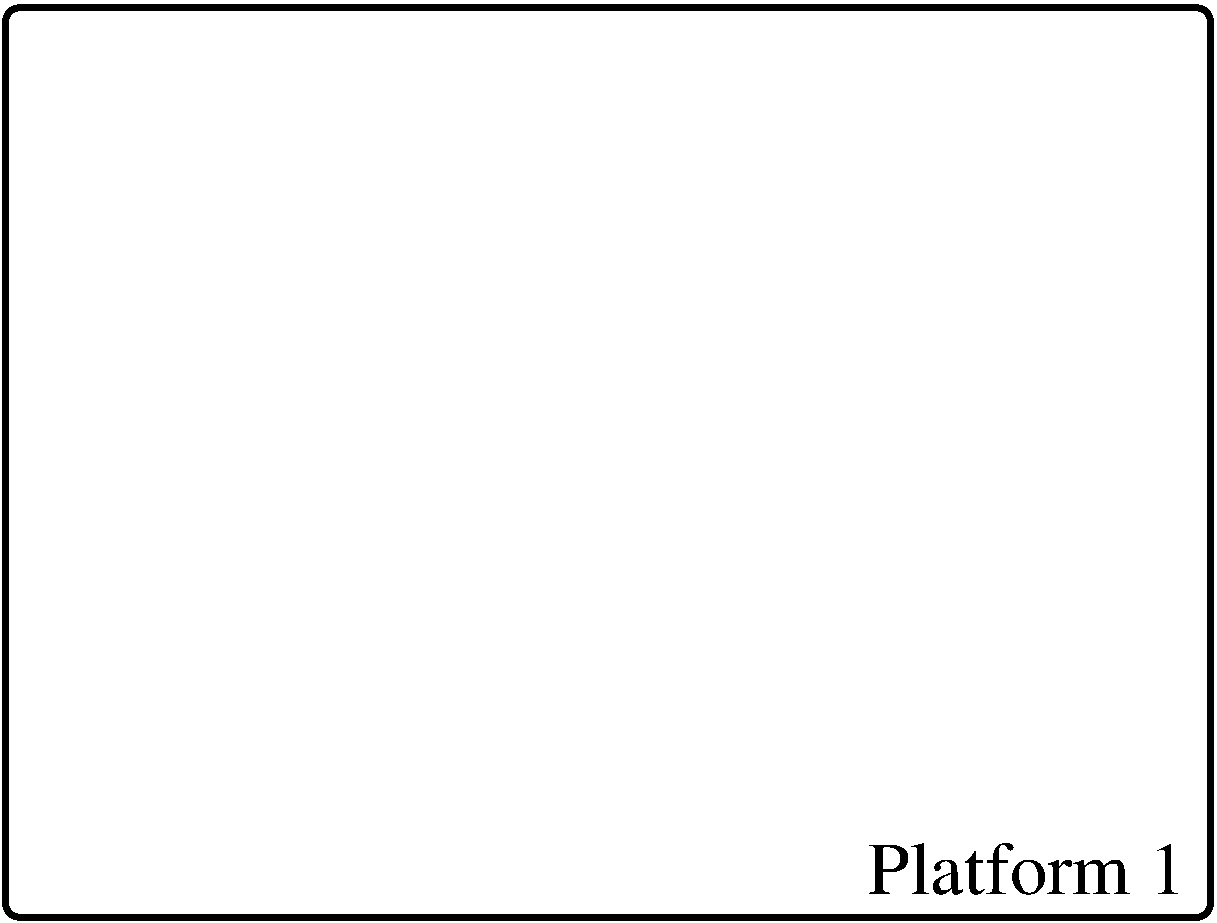
\includegraphics[width=0.85\textwidth]{figs/opencl-2.pdf}
 \end{center}
\end{frame}

\begin{frame}{OpenCL Platform Model}
 \begin{center}
   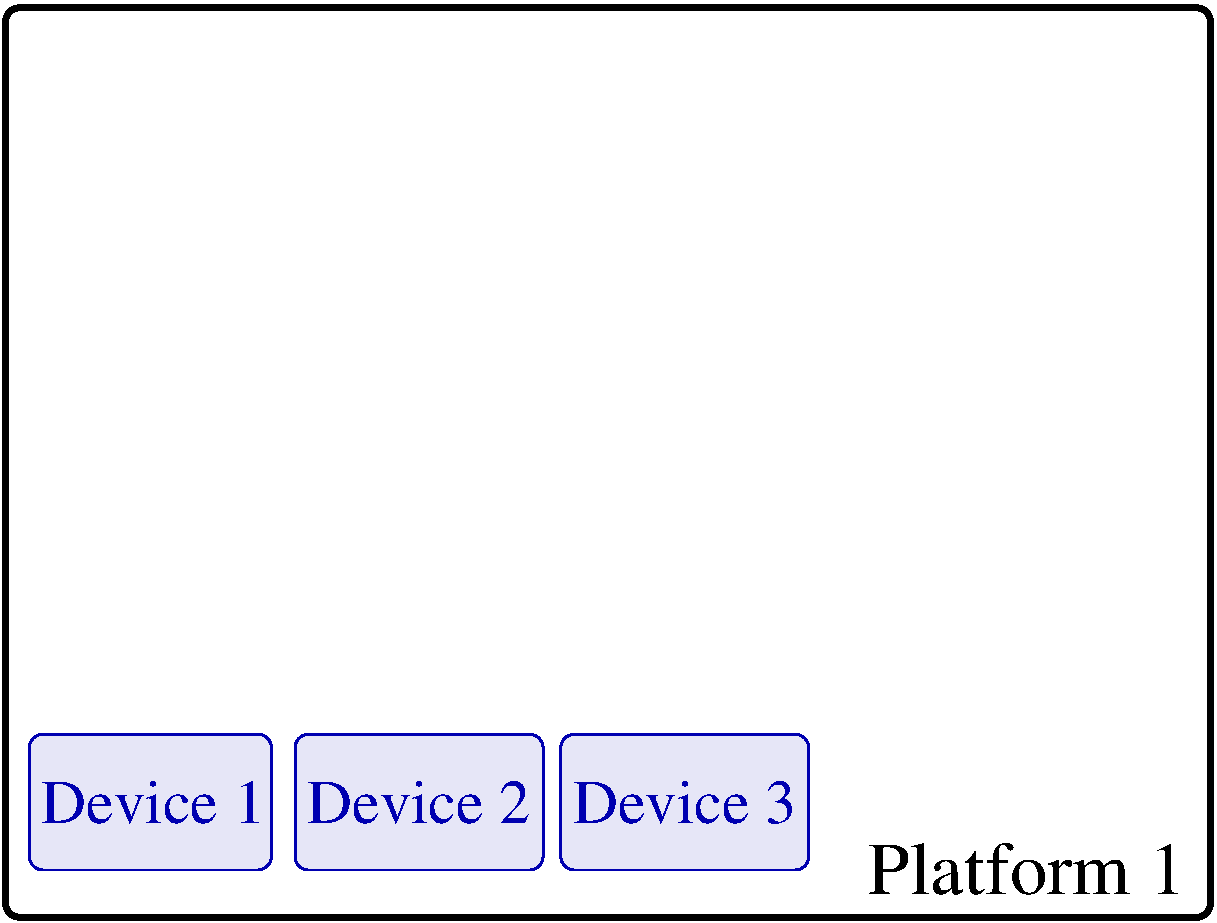
\includegraphics[width=0.85\textwidth]{figs/opencl-3.pdf}
 \end{center}
\end{frame}

\begin{frame}{OpenCL Platform Model}
 \begin{center}
   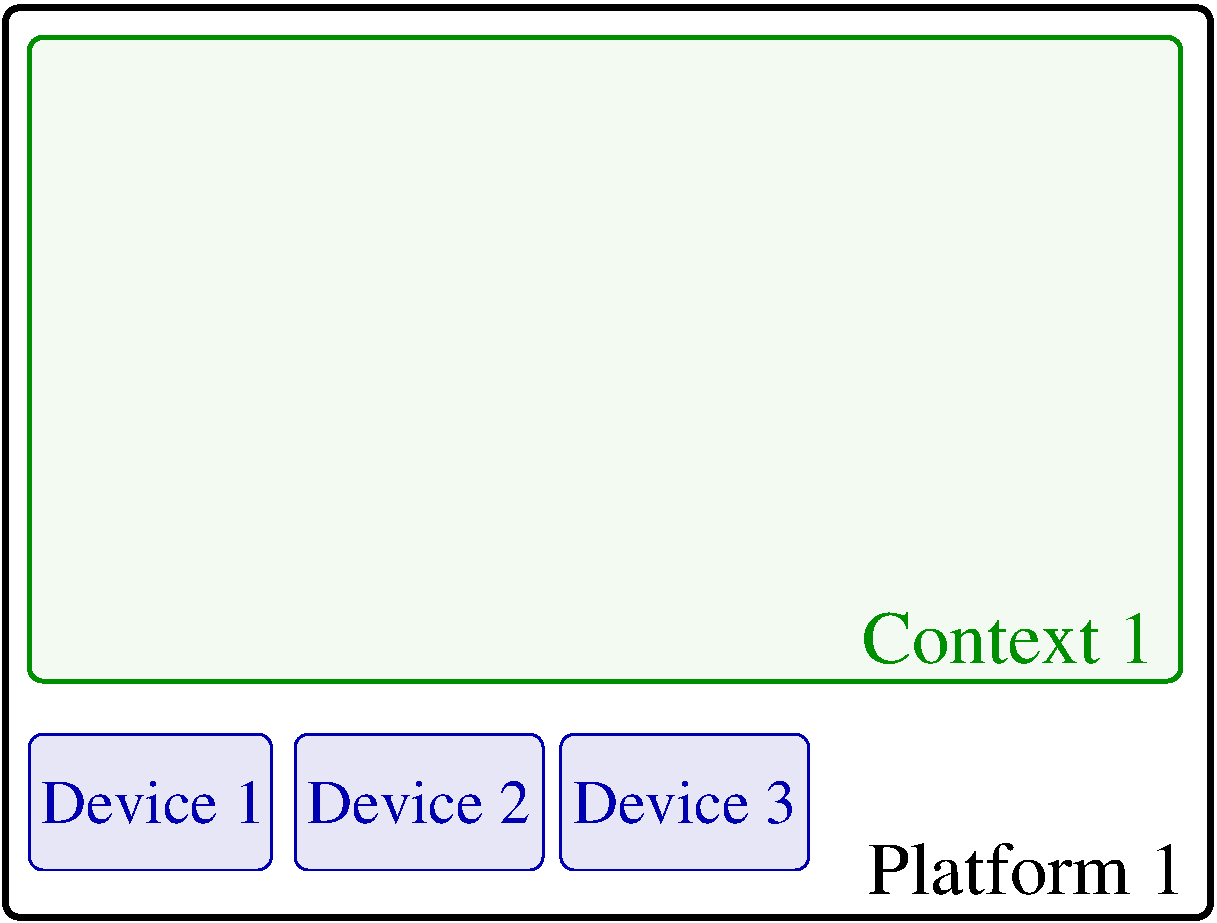
\includegraphics[width=0.85\textwidth]{figs/opencl-4.pdf}
 \end{center}
\end{frame}

\begin{frame}{OpenCL Platform Model}
 \begin{center}
   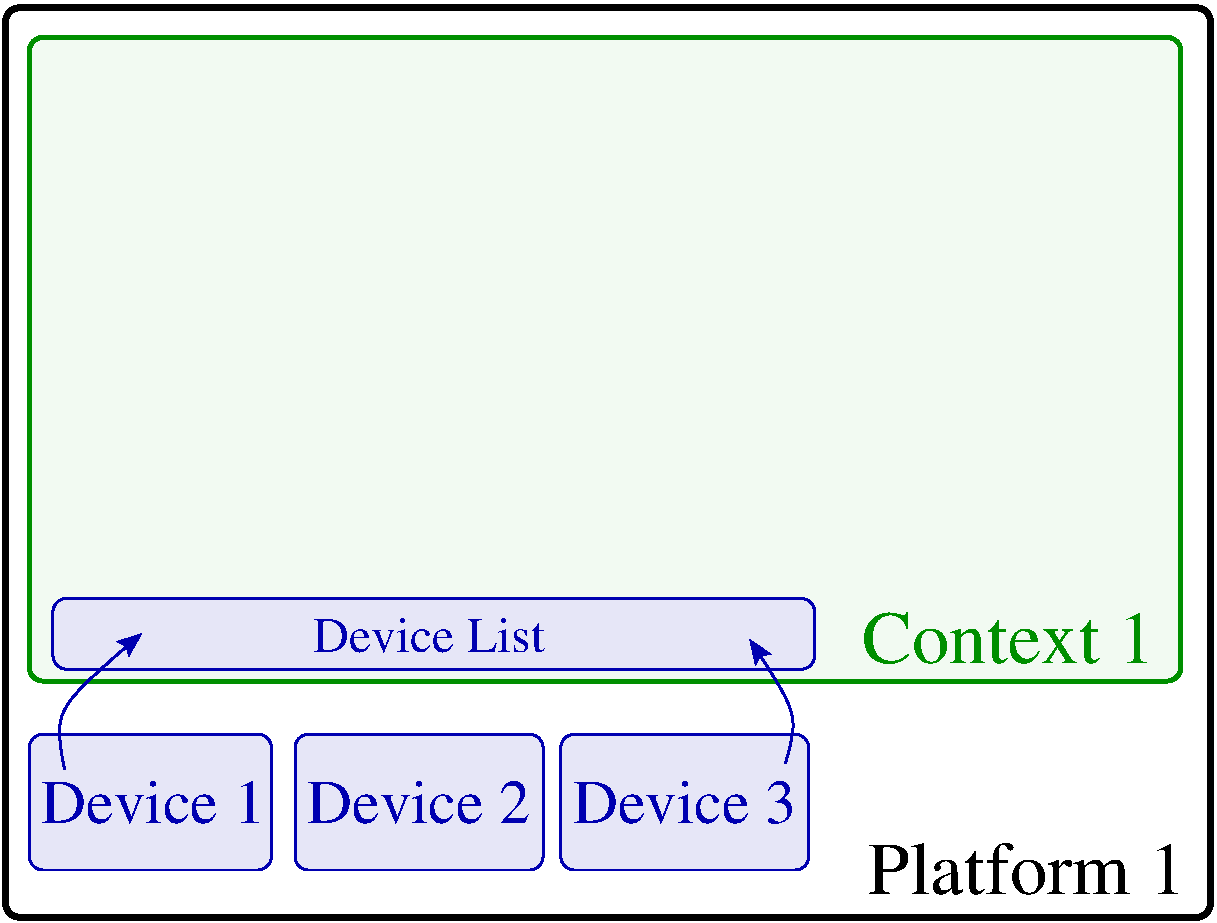
\includegraphics[width=0.85\textwidth]{figs/opencl-5.pdf}
 \end{center}
\end{frame}

\begin{frame}{OpenCL Platform Model}
 \begin{center}
   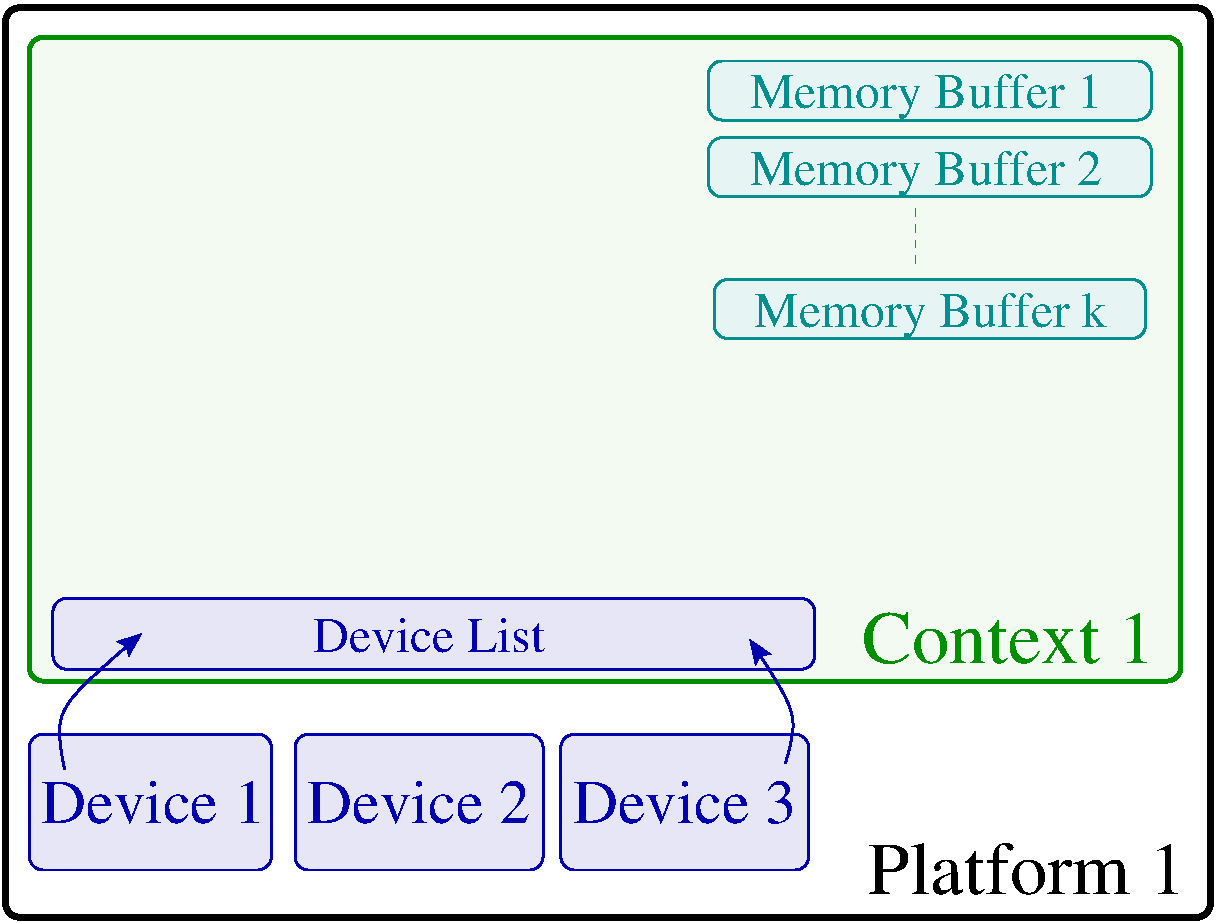
\includegraphics[width=0.85\textwidth]{figs/opencl-6.pdf}
 \end{center}
\end{frame}

\begin{frame}{OpenCL Platform Model}
 \begin{center}
   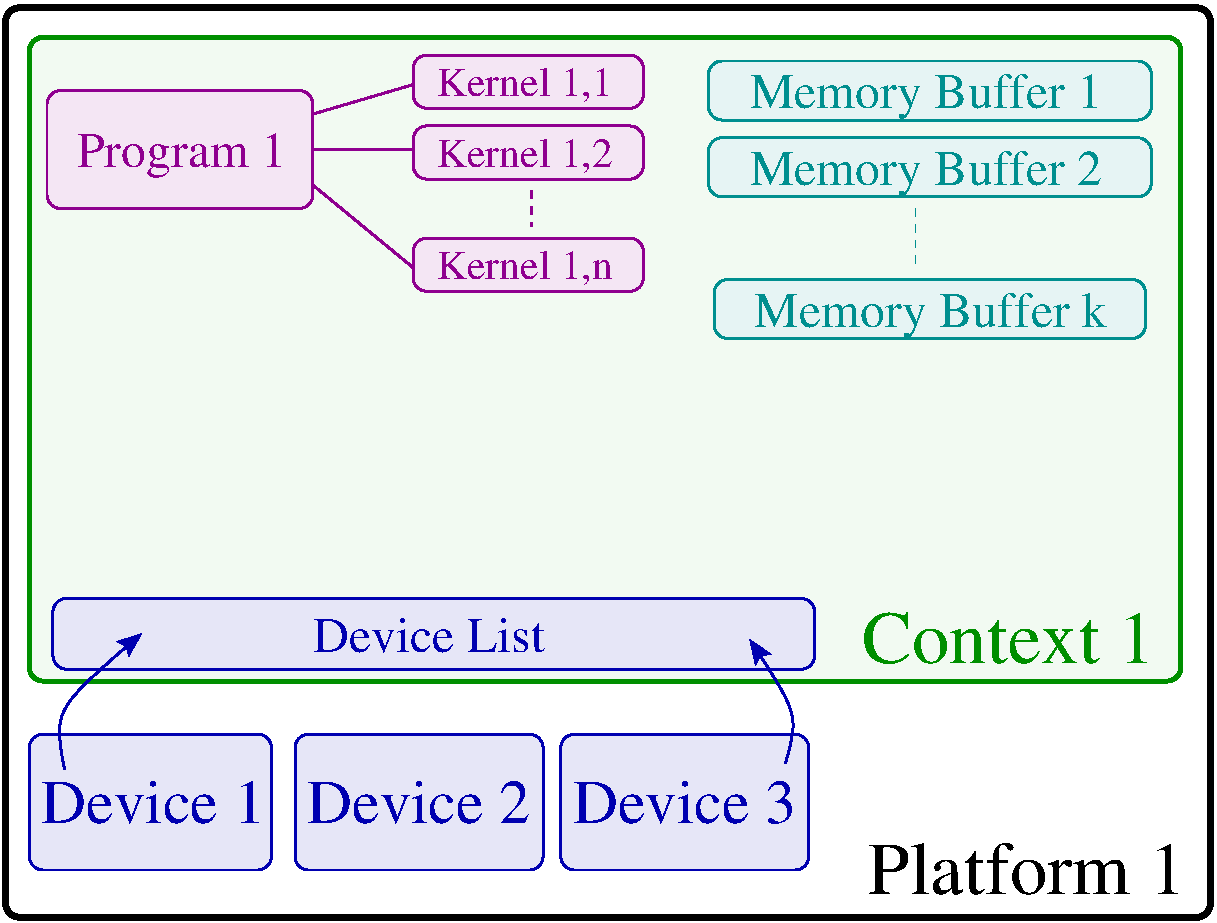
\includegraphics[width=0.85\textwidth]{figs/opencl-7.pdf}
 \end{center}
\end{frame}

\begin{frame}{OpenCL Platform Model}
 \begin{center}
   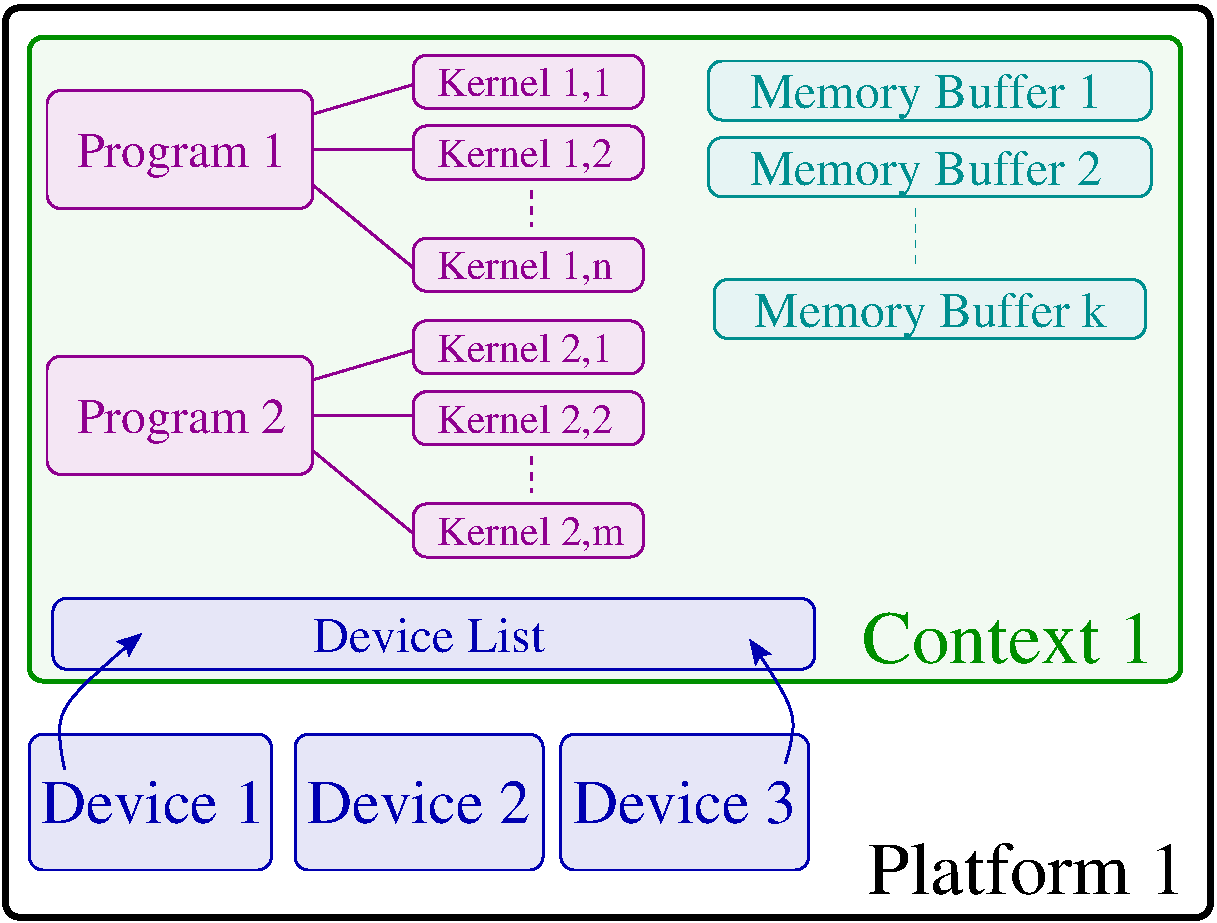
\includegraphics[width=0.85\textwidth]{figs/opencl-8.pdf}
 \end{center}
\end{frame}

\begin{frame}{OpenCL Platform Model}
 \begin{center}
   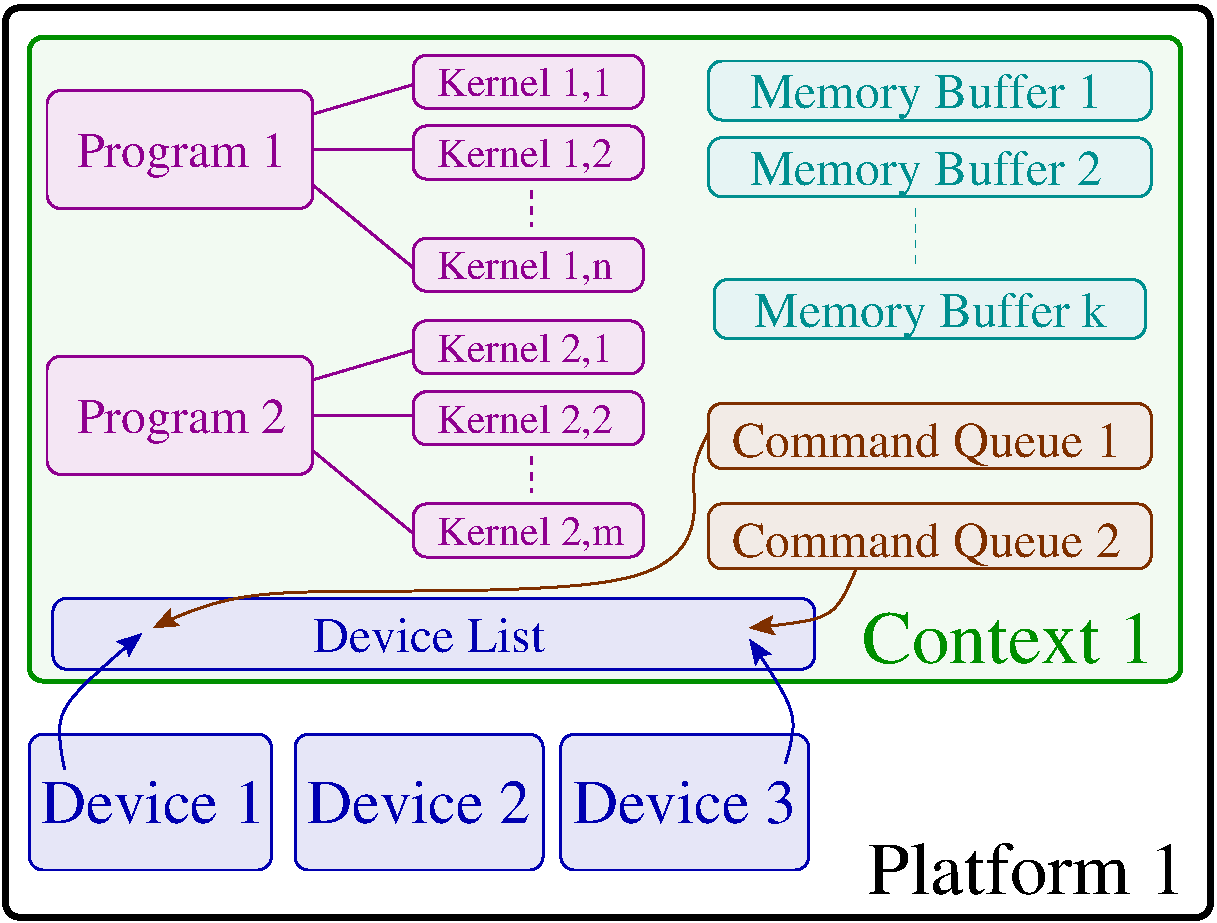
\includegraphics[width=0.85\textwidth]{figs/opencl-full.pdf}
 \end{center}
\end{frame}


%%%%%%%%%%%%%%%%%%%% Platform Model %%%%%%%%%%%%%%%%%%%%%%


\begin{frame}[fragile]
\frametitle{OpenCL Host API}

\lstset{ basicstyle=\scriptsize\ttfamily }
\begin{lstlisting}[escapechar=@]
@\color{red}{context}@ = clCreateContextFromType(NULL, CL_DEVICE_TYPE_GPU, NULL, NULL, NULL);
@\color{red}{queue}@ = clCreateCommandQueue(context, NULL, 0, NULL);
@\color{red}{memobjs[0]}@ = clCreateBuffer(context, CL_MEM_READ_WRITE, sizeof(float)*2*num_entries, NULL, NULL);
@\color{red}{memobjs[1]}@ = clCreateBuffer(context, CL_MEM_READ_ONLY | CL_MEM_COPY_HOST_PTR, sizeof(float)*2*num_entries, srcA, NULL);
 
@\color{red}{program}@ = clCreateProgramWithSource(context, 1, &kernel_src, NULL, NULL);
clBuildProgram(program, 0, NULL, NULL, NULL, NULL);
 
@\color{red}{kernel}@ = clCreateKernel(program, "my_kernel", NULL);
clSetKernelArg(kernel, 0, sizeof(cl_mem), (void *)&memobjs[0]);
clSetKernelArg(kernel, 1, sizeof(cl_mem), (void *)&memobjs[1]);
clSetKernelArg(kernel, 2, sizeof(float)*(local_work_size[0]+1)*16, NULL);
 
global_work_size[0] = 128;
 local_work_size[0] = 64;
clEnqueueNDRangeKernel(queue, kernel, 1, NULL, global_work_size, local_work_size, 0, NULL, NULL);
\end{lstlisting}
\lstset{ basicstyle=\small\ttfamily }

\begin{block}{Issues}
 \begin{itemize}
  \item ``Where is the error?''
  \item Manage OpenCL handles
 \end{itemize}

\end{block}

\end{frame}


\begin{frame}[fragile]
\frametitle{OpenCL Kernel Language}

\begin{block}{Sample Operation: Inplace Vector Addition}
 \vspace*{-0.5cm}
 \begin{align*}
  \left(
  \begin{array}{c}
   v_1^1 \\
   v_1^2 \\
   \vdots \\
   v_1^n 
  \end{array} \right) +\!= 
  \left(
  \begin{array}{c}
   v_2^1 \\
   v_2^2 \\
   \vdots \\
   v_2^n 
  \end{array} \right)
 \end{align*}
\end{block}

 \vspace*{-0.3cm}
\begin{block}{OpenCL Kernel}
\begin{lstlisting}
__kernel void inplace_add(
          __global const float * vec1,
          __global const float * vec2,
          unsigned int size) 
{ 
  for (unsigned int i  = get_global_id(0); 
                    i  < size; 
                    i += get_global_size(0))
    vec1[i] += vec2[i];
}
\end{lstlisting}
\end{block}

\end{frame}


%%%%%%%%%%%%%%%%% OpenCL closing %%%%%%%%%%%%%%%
% \begin{frame}{OpenCL Management}
%  \begin{center}
%    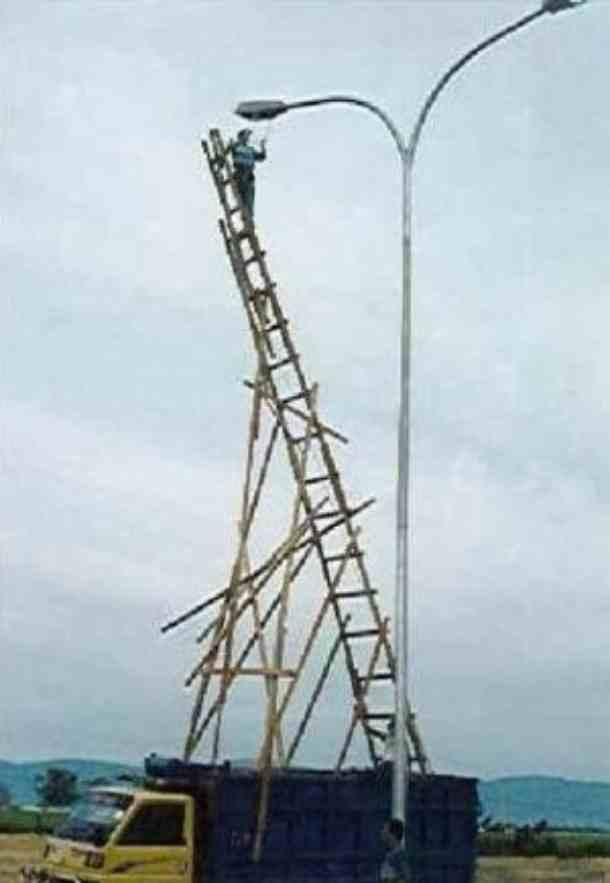
\includegraphics[width=0.45\textwidth]{figs/work1.jpg}
%  \end{center}
% \end{frame}






\begin{frame}{History of \ViennaCL}

\begin{block}{2010}
  \begin{itemize}
   \item April: Roots in the Master's Thesis of Florian Rudolf
   \item May 28th: ViennaCL 1.0.0 released
   \item November: 1000th download
   \item December: ViennaCL 1.1.0 \\(BLAS level 3, refurbished OpenCL backend)
  \end{itemize}
\end{block}

\vspace*{2.49cm}
\end{frame}



\begin{frame}{History of \ViennaCL}

\begin{block}{2010}
  \begin{itemize}
   \item April: Roots in the Master's Thesis of Florian Rudolf
   \item May 28th: ViennaCL 1.0.0 released
   \item November: 1000th download
   \item December: ViennaCL 1.1.0 \\(BLAS level 3, refurbished OpenCL backend)
  \end{itemize}
\end{block}

\begin{block}{2011}
  \begin{itemize}
   \item March: Accepted for Google Summer of Code
   \item December: ViennaCL 1.2.0 \\ (AMG, SPAI, FFT, QR, graph algorithms, structured matrices)
  \end{itemize}
\end{block}

\end{frame}



\begin{frame}{History of \ViennaCL}

\begin{block}{2012}
  \begin{itemize}
   \item March: Accepted for Google Summer of Code
   \item May: Tutorial at NVIDIA GTC 2012
   \item May: ViennaCL 1.3.0 \\ (ranges and slices, Automated OpenCL kernels, eigen values, ILU0, SVD)
   \item December: ViennaCL 1.4.0 \\ (CUDA and host backend, initializer types)
  \end{itemize}
\end{block}

\vspace{2.07cm}

\end{frame}


\begin{frame}{History of \ViennaCL}

\begin{block}{2012}
  \begin{itemize}
   \item March: Accepted for Google Summer of Code
   \item May: Tutorial at NVIDIA GTC 2012
   \item May: ViennaCL 1.3.0 \\ (ranges and slices, Automated OpenCL kernels, eigen values, ILU0, SVD)
   \item December: ViennaCL 1.4.0 \\ (CUDA and host backend, initializer types)
  \end{itemize}
\end{block}

\begin{block}{2013}
  \begin{itemize}
   \item May: Accepted for Google Summer of Code
   \item June: Tutorial at CGLibs
  \end{itemize}
\end{block}

\end{frame}


% \begin{frame}{History of \ViennaCL}
% 
% \TODO{Achievement unlocked: Historian}
% 
% \end{frame}



\begin{frame}{Goals of \ViennaCL}

  \begin{block}{About}
   \begin{itemize}
    \item High-level linear algebra C++ library
    \item OpenMP, OpenCL, and CUDA backends
    \item Header-only
    \item Multi-platform
   \end{itemize}
  \end{block}

  \vspace*{-2.3cm}
  \begin{flushright}
   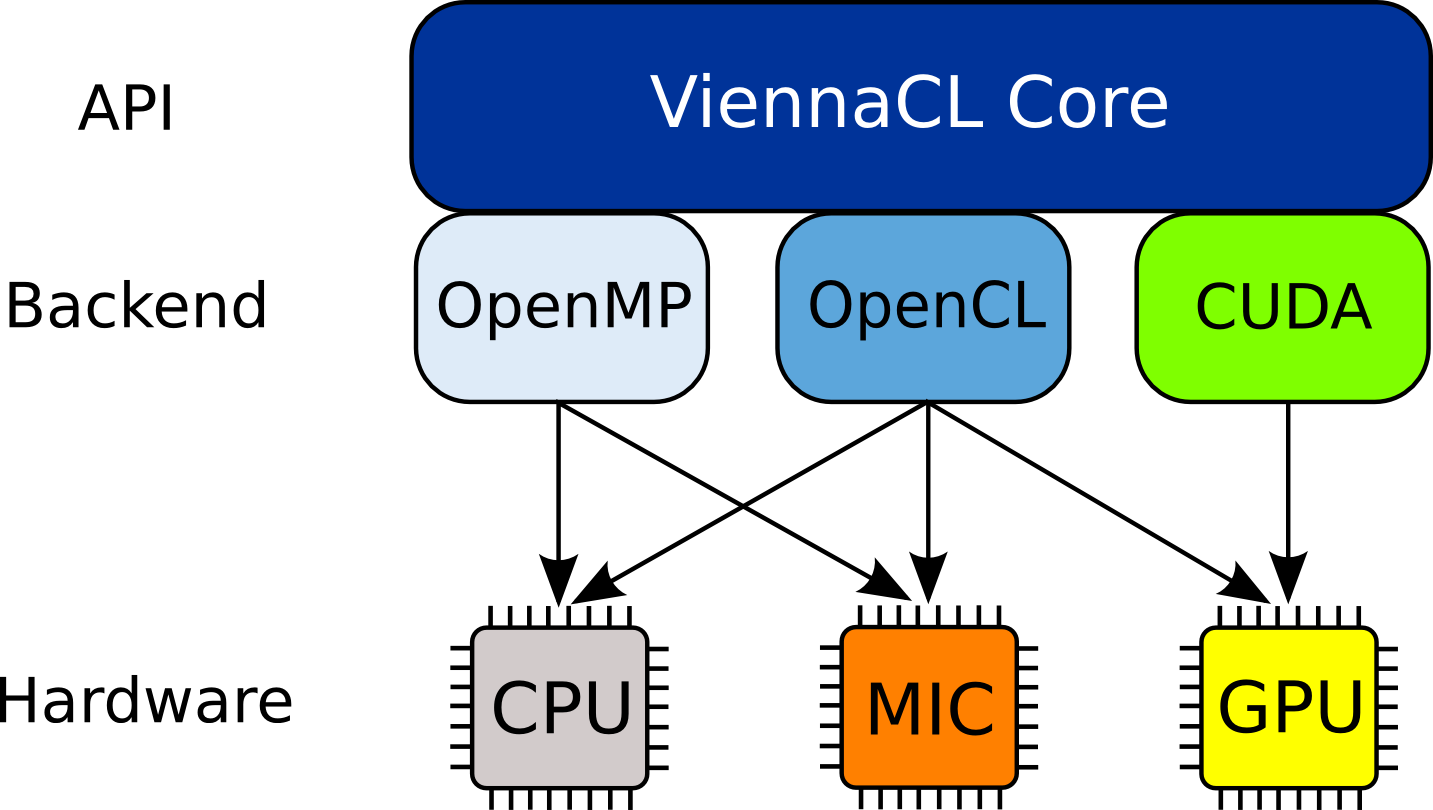
\includegraphics[width=0.4\textwidth]{figs/ViennaCL-arch.png}
  \end{flushright}

  \vspace*{-0.7cm}
  \begin{block}{Dissemination}
    \begin{itemize}
     \item Free Open-Source MIT (X11) License
     \item http://viennacl.sourceforge.net/
     \item 50-100 downloads per week
    \end{itemize}   
  \end{block}

  \begin{block}{Design Rules}
   \begin{itemize}
    \item Reasonable default values
    \item Compatible to Boost.uBLAS whenever possible 
    \item In doubt: clean design over performance
   \end{itemize}
  \end{block}

\end{frame}



\begin{frame}{Goals of \ViennaCL}

  \begin{block}{Core features}
    \begin{itemize}
     \item Linear algebra, BLAS
     \item Solver (direct and iterative)
     \item Preconditioners
    \end{itemize}   
  \end{block}
     
  \begin{block}{Additional features}
    \begin{itemize}
     \item Fast Fourier Transform
     \item Eigenvalue computations
     \item QR factorization
     \item Bandwidth reduction
     \item Nonnegative matrix factorization
    \end{itemize}   
  \end{block}

\end{frame}



\begin{frame}{Goals of \ViennaCL}

  \begin{block}{Interfaces to other libraries}
    \begin{itemize}
     \item Boost.uBLAS
     \item Eigen
     \item MTL4
    \end{itemize}   
  \end{block}

  \begin{block}{Backends}
   \begin{itemize}
    \item CPU
    \item OpenCL
    \item CUDA
   \end{itemize}
  \end{block}

  \begin{block}{C++ library}
   \begin{itemize}
    \item Generic free functions
    \item Expression templates
   \end{itemize}
  \end{block}

\end{frame}



\begin{frame}{Installation of \ViennaCL}

  \begin{block}{Three Steps}
    \begin{itemize}
     \item Download from http://viennacl.sourceforge.net/
     \item Unzip
     \item Copy source folder
    \end{itemize}   
  \end{block}

  \begin{block}{Dynamic Library?}
    \begin{itemize}
     \item ViennaCL is header-only
     \item Linking depends on used backend (OpenMP, OpenCL, CUDA)
    \end{itemize}
  \end{block}

  \begin{block}{Sample Applications}
    \begin{itemize}
     \item 22 tutorials
     \item $\hphantom{0}$7 benchmarks
     \item about 35 tests
    \end{itemize}
  \end{block}

\end{frame}



% ViennaCL Basics


%%%%%%%%%%%%%%%%%%%%%%%%%%%%%%%%%%% How-To: ViennaCL basics %%%%%%%%%%%%%%%%%%%%%%%%%%%%%%%%%%%%



\begin{frame}{ }
 \begin{center}
  \Large \textbf{How-To: \ViennaCL \ Basics}
 \end{center}
\end{frame}


\begin{frame}{How-To: \ViennaCL \ Basics}

\begin{block}{What to expect}
  \begin{itemize}
   \item From BLAS to Boost.uBLAS to ViennaCL
   \item Basic Types
   \item OpenCL Kernels
   \item Basic Usage: Data Management
   \item Basic Usage: Algebra
   \item Basic Usage: Solver
   \item Summary
  \end{itemize}
\end{block}

\end{frame}



\begin{frame}{From BLAS to Boost.uBLAS to ViennaCL}

\begin{block}{BLAS}
  \begin{itemize}
   \item \textbf{B}asic \textbf{L}inear \textbf{A}lgebra \textbf{S}ubprograms
   \item De facto API standard
   \item Low level interface
  \end{itemize}
\end{block}

\begin{block}{Boost.uBLAS}
  \begin{itemize}
   \item C++ API for BLAS
   \item High level interface
   \item Part of Boost libraries
  \end{itemize}
\end{block}

\end{frame}



\begin{frame}[fragile]
\frametitle{From BLAS to Boost.uBLAS to ViennaCL}
\begin{block}{Consider Existing CPU Code (Boost.uBLAS)}
  \begin{lstlisting}
using namespace boost::numeric::ublas;

matrix<double> A(1000, 1000);
vector<double> x(1000), rhs(1000);

/* Fill A, x, rhs here */

rhs += 2.0 * x;
double val = inner_prod(x, rhs);
matrix += val * outer_prod(x, rhs);

x = solve(A, rhs, upper_tag()); // Upper triangular solver

std::cout << "  2-norm: " << norm_2(x) << std::endl;
std::cout << "sup-norm: " << norm_inf(x) << std::endl;
  \end{lstlisting}
\end{block}

\begin{block}{High-Level Code with Syntactic Sugar}
\end{block}

\end{frame}


\begin{frame}{From BLAS to Boost.uBLAS to ViennaCL}

  \begin{block}{Porting the previous code to GPU}
  \end{block}

  \begin{block}{``How much time will you need{?}``}
    \begin{itemize}
     \item 1 minute?
     \item 1 hour?
     \item 1 day?
    \end{itemize}
  \end{block}

  \begin{block}{Quality Criteria}
   \begin{itemize}
     \item Working hours spent
     \item Performance
     \item Correctness
     \item High-level description (Maintainability)
   \end{itemize}
  \end{block}

\end{frame}


\begin{frame}[fragile]
\frametitle{From BLAS to Boost.uBLAS to ViennaCL}
\begin{block}{Consider Existing CPU Code (Boost.uBLAS)}
  \begin{lstlisting}
using namespace boost::numeric::ublas;


matrix<double> A(1000, 1000);
vector<double> x(1000), rhs(1000);

/* Fill A, x, rhs here */

rhs += 2.0 * x;
double val = inner_prod(x, rhs);
matrix += val * outer_prod(x, rhs);

x = solve(A, rhs, upper_tag()); // Upper triangular solver

std::cout << "  2-norm: " << norm_2(x) << std::endl;
std::cout << "sup-norm: " << norm_inf(x) << std::endl;
  \end{lstlisting}
\end{block}

\end{frame}

\begin{frame}[fragile]
\frametitle{From BLAS to Boost.uBLAS to ViennaCL}
 \begin{block}{Previous Code Snippet Rewritten with ViennaCL}
  \begin{lstlisting}
using namespace |\color{red}viennacl;|
using namespace |\color{red}viennacl::linalg;|

matrix<double> A(1000, 1000);
vector<double> x(1000), rhs(1000);

/* Fill A, x, rhs here */

rhs += 2.0 * x;
double val = inner_prod(x, rhs);
matrix += val * outer_prod(x, rhs);

x = solve(A, rhs, upper_tag()); // Upper triangular solver

std::cout << "  2-norm: " << norm_2(x) << std::endl;
std::cout << "sup-norm: " << norm_inf(x) << std::endl;
  \end{lstlisting} 
 \end{block}
\end{frame}



%%%%%%%%%%%%%%% Iterative solvers %%%%%%%%%%%%%%%%%%%%%%
\begin{frame}[fragile]
\frametitle{From BLAS to Boost.uBLAS to ViennaCL}
\begin{block}{ViennaCL in addition provides iterative solvers}
  \begin{lstlisting}
using namespace viennacl;
using namespace viennacl::linalg;

compressed_matrix<double> A(1000, 1000);
vector<double> x(1000), rhs(1000);

/* Fill A, x, rhs here */

x = solve(A, rhs, cg_tag()); // Conjugate Gradient solver
x = solve(A, rhs, bicgstab_tag()); // BiCGStab solver
x = solve(A, rhs, gmres_tag());    // GMRES solver
  \end{lstlisting}
\end{block}

 \begin{block}{No iterative solvers available in uBLAS...}
 \end{block}
\end{frame}


\begin{frame}[fragile]
\frametitle{From BLAS to Boost.uBLAS to ViennaCL}
\begin{block}{Thanks to interface compatibility}
  \begin{lstlisting}
using namespace |\color{red}boost::numeric::ublas;|
using namespace viennacl::linalg;

compressed_matrix<double> A(1000, 1000);
vector<double> x(1000), rhs(1000);

/* Fill A, x, rhs here */

x = solve(A, rhs, cg_tag()); // Conjugate Gradient solver
x = solve(A, rhs, bicgstab_tag()); // BiCGStab solver
x = solve(A, rhs, gmres_tag());    // GMRES solver
  \end{lstlisting} 
\end{block}

\vspace{1.15cm}

\end{frame}



\begin{frame}[fragile]
\frametitle{OpenCL kernels}

\begin{block}{OpenCL kernels are needed for actual computation}
  \begin{itemize}
   \item Provided by ViennaCL
   \item Support for expression templates
   \item Automatic kernel generation
  \end{itemize}
\end{block}

\begin{block}{Each of the following commands launches a separate OpenCL kernel}
\begin{lstlisting}
v1 = v2;
v1 += v2;
v1 -= v2;
v1 = alpha * v2;
v1 += alpha * v2;
v1 -= alpha * v2;
v1 *= alpha;
v1 /= alpha;
\end{lstlisting}
\end{block}

\end{frame}


\begin{frame}[fragile]
\frametitle{OpenCL kernels}

\begin{block}{OpenCL kernels have to be compiled at run time}
\begin{itemize}
  \item OpenCL JIT compiler
  \item Kernels can be grouped in programs
\end{itemize}
\end{block}

\begin{block}{Compilation strategies}
\begin{itemize}
  \item Each kernel individually: several milliseconds per kernel
  \item All at once: Takes seconds
  \item In groups: Compile groups of kernels whenever potentially needed
\end{itemize}
\end{block}

\end{frame}


\begin{frame}[fragile]
\frametitle{OpenCL kernels}

\begin{block}{Consider the following code}
  \begin{lstlisting}
int main(){
  vector<double> x(100), y(100);
  matrix<double> A(100, 100), B(100, 100);
  matrix<double, column_major> C(100, 100);

  x += 3.1415 * y;
  C = prod(trans(A), B);
  y = prod(C, x);

  std::cout << y << std::endl;
}
  \end{lstlisting}
\end{block}

\begin{block}{OpenCL Kernels}
  \begin{itemize}
    \item Which kernels are compiled?
    \item When are they compiled?
    \item Hint: Program compiles and executes normally
  \end{itemize}
\end{block}

\end{frame}


\begin{frame}[fragile]
\frametitle{OpenCL kernels}

\begin{block}{Consider the following code}
  \begin{lstlisting}
int main(){
  |\color{red}vector<double> x(100), y(100);|
  |\color{red}matrix<double> A(100, 100), B(100, 100);|
  |\color{red}matrix<double, column\_major> C(100, 100);|

  x += 3.1415 * y;
  C = prod(trans(A), B);
  y = prod(C, x);

  std::cout << y << std::endl;
}
  \end{lstlisting}
\end{block}

\begin{block}{OpenCL Kernels}
  \begin{itemize}
    \item Which kernels are compiled?
    \item When are they compiled?
    \item Hint: Program compiles and executes normally
  \end{itemize}
\end{block}

\end{frame}



\begin{frame}[fragile]
\frametitle{OpenCL kernels}

\begin{block}{Consider the following code}
  \begin{lstlisting}
int main(){
  vector<double> x(100), y(100);
  matrix<double> A(100, 100), B(100, 100);
  matrix<double, column_major> C(100, 100);

  |\color{red}x += 3.1415 * y;|
  |\color{red}C = prod(trans(A), B);|
  |\color{red}y = prod(C, x);|

  std::cout << y << std::endl;
}
  \end{lstlisting}
\end{block}

\begin{block}{OpenCL Kernels}
  \begin{itemize}
    \item Which kernels are compiled?
    \item When are they compiled?
    \item Hint: Program compiles and executes normally
  \end{itemize}
\end{block}

\end{frame}


\begin{frame}{OpenCL kernel management}

\begin{block}{Special case: Matrix-Matrix product}
  \begin{itemize}
    \item Result matrix: Row/Column major memory layout
    \item First factor: Row/Column major, possibly transposed
    \item Second factor: Row/Column major, possibly transposed
  \end{itemize}
\end{block}

\begin{block}{Leads to 32 different kernels for matrix-matrix multiplication}
  \begin{itemize}
    \item Compiled separately on request
  \end{itemize}
\end{block}

\end{frame}



\begin{frame}{Basic Types}

\begin{block}{Supported types}
  \begin{itemize}
   \item Scalar
   \item Vector
   \item Dense matrix
   \item Sparse matrix
   \item Structured matrix
  \end{itemize}
\end{block}

\begin{block}{Numeric Types}
  \begin{itemize}
   \item float
   \item double
  \end{itemize}
\end{block}

\end{frame}



% \begin{frame}{Basic Types}
% 
% \TODO{Bild overview over types (scalar, vectors, matrices, dense matrices, sparse matrices, special types, ...)}
% 
% \end{frame}



\begin{frame}[fragile]
\frametitle{Basic Types}

\begin{block}{Scalars}  
  \begin{itemize}
   \item Represents a single scalar value on the computing device
   \item Behave like underlying type
   \item Implicit cast to underlying type
   \item Potentially expensive (Overhead!)
  \end{itemize}
  
  \begin{lstlisting}
viennacl::scalar<NumericType> gpu_scalar;
viennacl::scalar<float> gpu_float;
viennacl::scalar<double> gpu_double;
  \end{lstlisting}
\end{block}

\end{frame}



\begin{frame}[fragile]
\frametitle{Basic Types}
\begin{block}{Scalars}
  \begin{lstlisting}
float cpu_float = 42.0f;
double cpu_double = 13.7603;
viennacl::scalar<float> gpu_float(3.1415f);
viennacl::scalar<double> gpu_double = 2.71828;

// conversions and t
cpu_float = gpu_float;
// automatic transfer and conversion
gpu_float = cpu_double;

cpu_float = gpu_float * 2.0f;
cpu_double = gpu_float - cpu_float;
  \end{lstlisting}
\end{block}
\end{frame}



\begin{frame}[fragile]
\frametitle{Basic Types}

\begin{block}{Vectors}  
  \begin{itemize}
   \item Represents a vector on the computing device
   \item Operator overloading
   \item Alignment support
  \end{itemize}
  
  \begin{lstlisting}
viennacl::vector<NumericType> gpu_vector;

viennacl::vector<float> gpu_float_vector;
viennacl::vector<double> gpu_double_vector;
  \end{lstlisting}
\end{block}

\end{frame}



\begin{frame}[fragile]
\frametitle{Basic Types}

\begin{block}{Vectors}
  \begin{lstlisting}
std::vector<ScalarType> stl_vec(10);
viennacl::vector<ScalarType> vcl_vec(10);

//fill the STL vector:
for (unsigned int i=0; i<vector_size; ++i)
  stl_vec[i] = i;

//copy content to GPU vector (recommended initialization)
copy(stl_vec.begin(), stl_vec.end(), vcl_vec.begin());

//manipulate GPU vector here
vcl_vec *= 4.2;

//copy content from GPU vector back to STL vector
copy(vcl_vec.begin(), vcl_vec.end(), stl_vec.begin());
  \end{lstlisting}
\end{block}

\end{frame}



\begin{frame}[fragile]
\frametitle{Basic Types}

\begin{block}{Vectors}
  \begin{lstlisting}
std::vector<ScalarType> stl_vec(10);
viennacl::vector<ScalarType> vcl_vec(10);

//fill the STL vector:
for (unsigned int i=0; i<vector_size; ++i)
  stl_vec[i] = i;

//copy content to GPU vector (recommended initialization)
copy(stl_vec, vcl_vec);

//manipulate GPU vector here
vcl_vec *= 4.2;

//copy content from GPU vector back to STL vector
copy(vcl_vec, stl_vec);
  \end{lstlisting}
\end{block}

\end{frame}




\begin{frame}[fragile]
\frametitle{Basic Types}

\begin{block}{Alignment}  
  \begin{itemize}
   \item Default = 1
   \item Template parameter
   \item In ViennaCL 1.5.0 deprecated (will be runtime parameter)
  \end{itemize}
  
  \begin{lstlisting}
viennacl::vector<NumericType, Alignment> gpu_vector_with_alignment;

viennacl::vector<float, 4>
    gpu_float_vector_with_alignment;

viennacl::vector<double, 8>
    gpu_double_vector_with_alignment;
  \end{lstlisting}
\end{block}

\end{frame}



\begin{frame}[fragile]
\frametitle{Basic Types}

\begin{block}{Vector initializer}  
  \begin{itemize}
   \item unit\_vector $\Rightarrow \textbf{u}_{N,i} = \left\{ \begin{array}{ll} 1 & \mbox{if $i = N$}; \\
                                                                     0 &  \mbox{else} \end{array} \right.$
   \item zero\_vector $\Rightarrow \textbf{z}_i = 0$
   \item scalar\_vector $\Rightarrow \textbf{s}_i = s$
  \end{itemize}
  
  \begin{lstlisting}
viennacl::unit_vector<NumericType>(size, index);
    
viennacl::zero_vector<NumericType>(size);
    
viennacl::scalar_vector<NumericType>(size, scalar);
  \end{lstlisting}
\end{block}

\end{frame}



\begin{frame}[fragile]
\frametitle{Basic Types}

\begin{block}{Vector initializer}
  \begin{lstlisting}
viennacl::vector<ScalarType> vcl_vec =
    viennacl::unit_vector<ScalarType>(10, 5);
// Creates the vector (0, 0, 0, 0, 1, 0, 0, 0, 0, 0)

viennacl::vector<ScalarType> vcl_vec =
    viennacl::zero_vector<ScalarType>(10);
// Creates the vector (0, 0, 0, 0, 0, 0, 0, 0, 0, 0)

viennacl::vector<ScalarType> vcl_vec =
    viennacl::scalar_vector<ScalarType>(6, 1.5);
// Creates the vector (1.5, 1.5, 1.5, 1.5, 1.5, 1.5)
  \end{lstlisting}
\end{block}

\end{frame}



\begin{frame}[fragile]
\frametitle{Basic Types}

\begin{block}{Dense matrix}  
  \begin{itemize}
   \item Represents a dense matrix on the computing device
   \item Dense matrix $\Rightarrow$ zero elements are rare
   \item Alignment support (same as vectors)
   \item Row major or column major
  \end{itemize}
  
  \begin{lstlisting}
viennacl::matrix<NumericType> gpu_matrix;
viennacl::matrix<NumericType, Scheme, Alignment>
    gpu_matrix_with_scheme_and_alignment;

viennacl::matrix<float> gpu_float_matrix;
viennacl::matrix<float, row_major, 4>
    row_major_gpu_float_matrix_with_alignment;

viennacl::matrix<double> gpu_double_matrix;
viennacl::matrix<double, column_major, 8>
    column_major_gpu_double_matrix_with_alignment;
  \end{lstlisting}
\end{block}

\end{frame}




\begin{frame}[fragile]
\frametitle{Basic Types}

\begin{block}{Dense matrix}
  \begin{lstlisting}
//set up a 3 by 5 matrix:
viennacl::matrix<float> vcl_matrix(4, 5);
//fill it up:
vcl_matrix(0,2) =  1.0
vcl_matrix(1,2) = -1.5;
vcl_matrix(2,0) =  4.2;
vcl_matrix(3,4) =  3.1415;
  \end{lstlisting}
\end{block}

\end{frame}



\begin{frame}[fragile]
\frametitle{Basic Types}

\begin{block}{Matrix initializer}  
  \begin{itemize}
   \item identity\_matrix $\Rightarrow \textbf{I}_{i,j} = \left\{ \begin{array}{ll} d & \mbox{if $i = j$}; \\
                                                                     0 &  \mbox{else} \end{array} \right.$
   \item zero\_matrix $\Rightarrow \textbf{Z}_{i,j} = 0$
   \item scalar\_matrix $\Rightarrow \textbf{S}_{i,j} = s$
  \end{itemize}
  
  \begin{lstlisting}
viennacl::identity_matrix<NumericType>(size, diagonal);
    
viennacl::zero_matrix<NumericType>(row_number, column_number);
    
viennacl::scalar_matrix<NumericType>(row_number, column_number, scalar);
  \end{lstlisting}
\end{block}

\end{frame}



\begin{frame}[fragile]
\frametitle{Basic Types}

\begin{block}{Matrix initializer}
  \begin{lstlisting}
viennacl::matrix<ScalarType> vcl_mat =
    viennacl::identity_matrix<ScalarType>(4, 1);
  \end{lstlisting}
  
  \hspace{1cm}
  
  Creates the following matrix:
$\begin{pmatrix}
1 & 0 & 0 & 0 \\
0 & 1 & 0 & 0 \\
0 & 0 & 1 & 0 \\
0 & 0 & 0 & 1
\end{pmatrix}$
\end{block}

\end{frame}



\begin{frame}[fragile]
\frametitle{Basic Types}

\begin{block}{Matrix initializer}
  \begin{lstlisting}
viennacl::matrix<ScalarType> vcl_mat =
    viennacl::zero_matrix<ScalarType>(3, 5);
  \end{lstlisting}
  
  \hspace{1cm}
  
  Creates the following matrix:
$\begin{pmatrix}
0 & 0 & 0 & 0 & 0 & 0 \\
0 & 0 & 0 & 0 & 0 & 0 \\
0 & 0 & 0 & 0 & 0 & 0
\end{pmatrix}$
\end{block}

\end{frame}



\begin{frame}[fragile]
\frametitle{Basic Types}

\begin{block}{Matrix initializer}
  \begin{lstlisting}
viennacl::matrix<ScalarType> vcl_mat =
    viennacl::scalar_matrix<ScalarType>(4, 3, 4.2);
  \end{lstlisting}
  
  \hspace{1cm}
  
  Creates the following matrix:
$\begin{pmatrix}
4.2 & 4.2 & 4.2 \\
4.2 & 4.2 & 4.2 \\
4.2 & 4.2 & 4.2 \\
4.2 & 4.2 & 4.2
\end{pmatrix}$
\end{block}

\end{frame}



\begin{frame}
\frametitle{Basic Types}

\begin{block}{Sparse matrix}
  \begin{itemize}
   \item Represents a sparse matrix on the computing device
   \item Sparse matrix $\Rightarrow$ zero elements are frequent
   \item Alignment support (same as vectors and dense matrices)
  \end{itemize}
\end{block}


\begin{block}{Sparse matrix types}
  \begin{itemize}
   \item Coordinate matrix
   \item Compressed matrix
   \item ELL matrix
   \item Hybrid matrix
  \end{itemize}
\end{block}

\end{frame}



\begin{frame}
\frametitle{Basic Types}

\begin{block}{Coordinate matrix}
  \begin{itemize}
   \item Easy to setup/extend
  \end{itemize}
  
  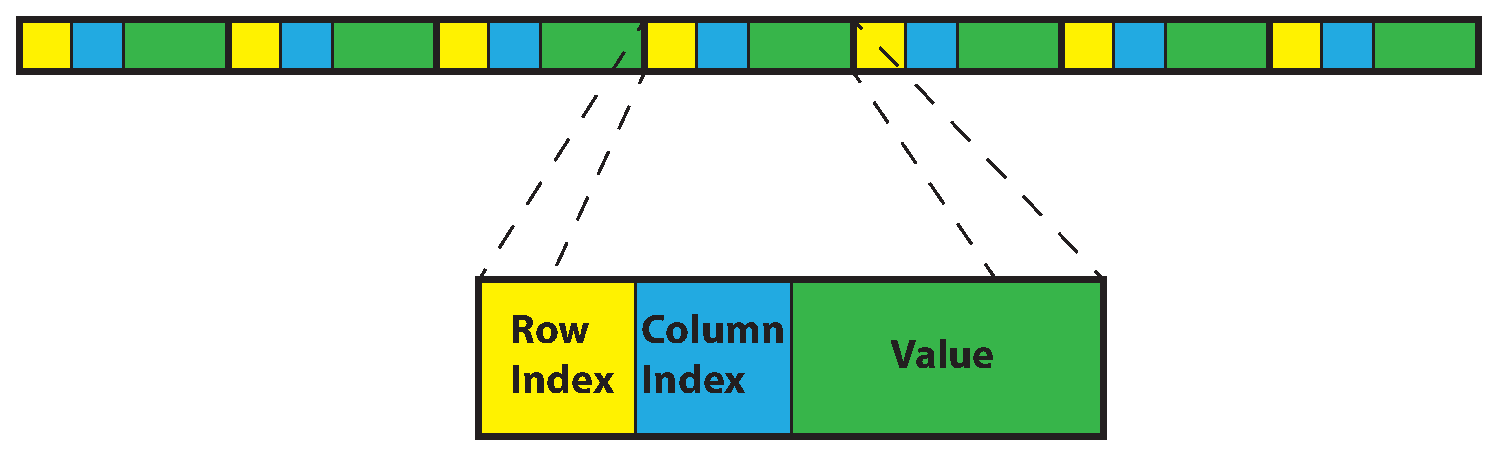
\includegraphics[width=0.8\textwidth]{figs/coordinate_matrix.eps}
\end{block}

\end{frame}



\begin{frame}
\frametitle{Basic Types}

\begin{block}{Compressed matrix}
  \begin{itemize}
    \item Less memory required
    \item Fast matrix-vector multiplication
  \end{itemize}
  
  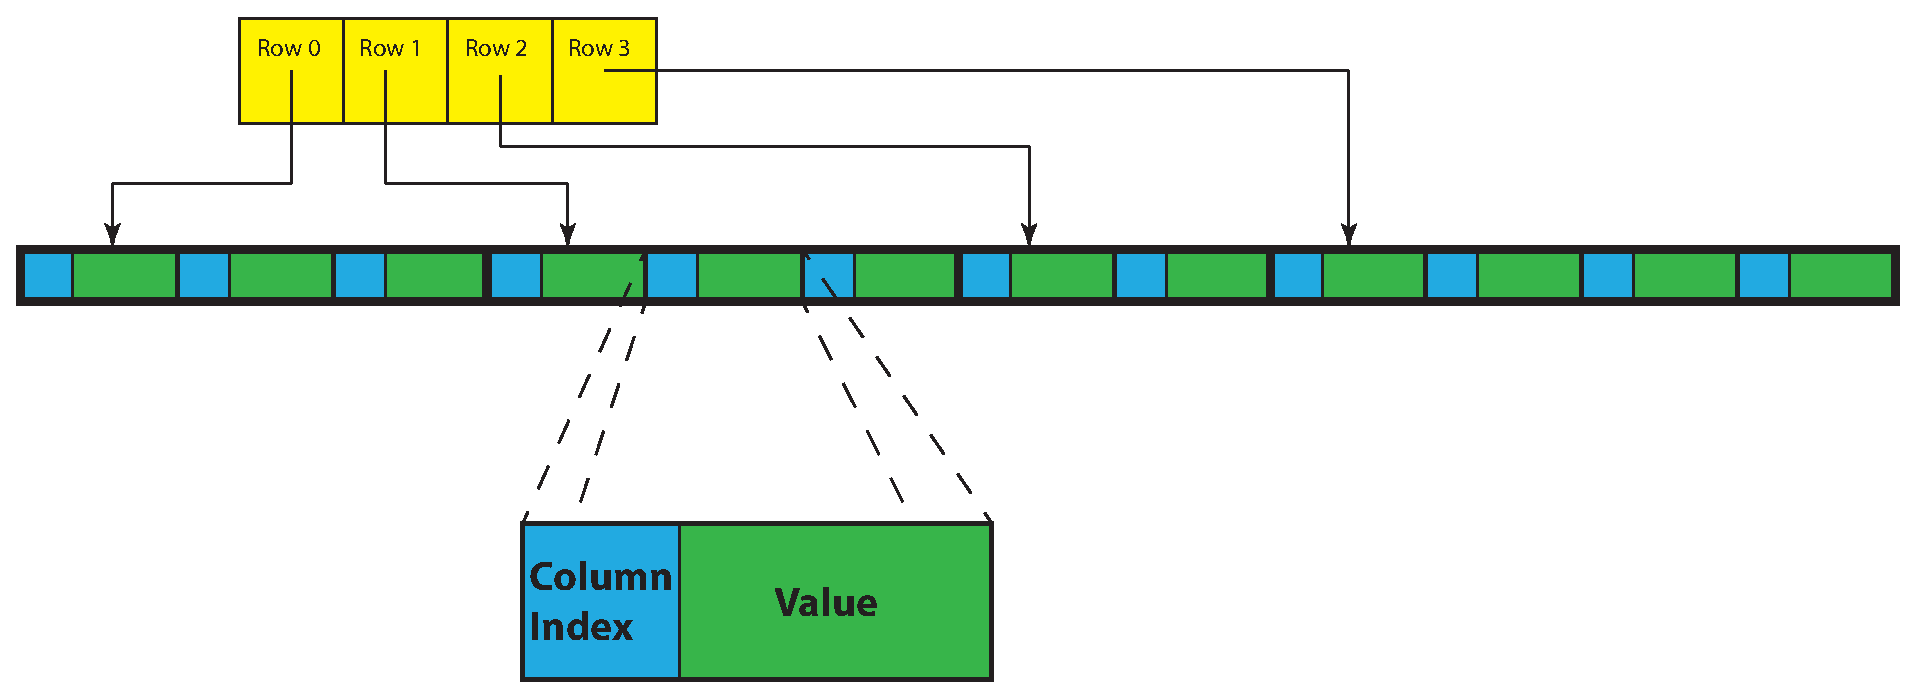
\includegraphics[width=0.8\textwidth]{figs/compressed_matrix.eps}
\end{block}

\end{frame}


\begin{frame}
\frametitle{Basic Types}

\begin{block}{ELL matrix}
  \begin{itemize}
    \item Similar to compressed matrix
    \item Fixed number of non-zero values per row
    \item No row jumper array required
  \end{itemize}
\end{block}

\begin{block}{Hybrid matrix}
  \begin{itemize}
    \item Combination of compressed matrix and ELL matrix
  \end{itemize}
\end{block}

\end{frame}



\begin{frame}[fragile]
\frametitle{Basic Types}

\begin{block}{Compressed matrix}
  \begin{lstlisting}
//set up a sparse 4 by 5 matrix on the CPU:
std::vector< std::map< unsigned int, float> >
    cpu_sparse_matrix(4);

//fill it up:
cpu_sparse_matrix[0][2] = 1.0;
cpu_sparse_matrix[1][2] = -1.5;
cpu_sparse_matrix[3][0] = 4.2;

//set up a sparse ViennaCL matrix:
viennacl::compressed_matrix<float> sparse_matrix(4, 5);

//copy to OpenCL device:
copy(cpu_sparse_matrix, sparse_matrix);

//copy back to CPU:
copy(sparse_matrix, cpu_sparse_matrix);
  \end{lstlisting}
\end{block}

\end{frame}





\begin{frame}
\frametitle{Basic Types}

\begin{block}{Structured matrix}
  \begin{itemize}
   \item Dense matrices but with special structure
   \item Access to one element might change other elements
  \end{itemize}
\end{block}

\begin{block}{Supported types}
  \begin{itemize}
   \item Circulant matrix
   \item Hankel matrix
   \item Toeplitz matrix
   \item Vandermonde matrix
  \end{itemize}
\end{block}

\end{frame}


\begin{frame}
\frametitle{Basic Types}

\begin{block}{Structured matrix}
  \begin{itemize}
   \item \textbf{Circulant matrix}
   \item Hankel matrix
   \item Toeplitz matrix
   \item Vandermonde matrix
  \end{itemize}
\end{block}

\begin{align*}
 \left( \begin{array}{ccccc}
         c_0 & c_{n-1} & \ldots & c_2 & c_1 \\
         c_1 & c_0 & c_{n-1} & & c_2 \\
         \vdots & c_1 & c_0 & \ddots & \vdots \\
         c_{n-2} & & \ddots & \ddots & c_{n-1} \\
         c_{n-1} & c_{n-2} & \hdots & c_1 & c_0 \\
        \end{array} \right)
\end{align*}

\end{frame}



\begin{frame}
\frametitle{Basic Types}

\begin{block}{Structured matrix}
  \begin{itemize}
   \item Circulant matrix
   \item \textbf{Hankel matrix}
   \item Toeplitz matrix
   \item Vandermonde matrix
  \end{itemize}
\end{block}

\begin{align*}
 \left( \begin{array}{cccc}
         a & b & c & d \\
         b & c & d & e \\
         c & d & e & f \\
         d & e & f & g \\
        \end{array} \right)
\end{align*}

\vspace{0.9cm}

\end{frame}


\begin{frame}
\frametitle{Basic Types}

\begin{block}{Structured matrix}
  \begin{itemize}
   \item Circulant matrix
   \item Hankel matrix
   \item \textbf{Toeplitz matrix}
   \item Vandermonde matrix
  \end{itemize}
\end{block}

\begin{align*}
 \left( \begin{array}{cccc}
         a & b & c & d \\
         e & a & b & c \\
         f & e & a & b \\
         g & f & e & a \\
        \end{array} \right)
\end{align*}

\vspace{0.9cm}

\end{frame}



\begin{frame}
\frametitle{Basic Types}

\begin{block}{Structured matrix}
  \begin{itemize}
   \item Circulant matrix
   \item Hankel matrix
   \item Toeplitz matrix
   \item \textbf{Vandermonde matrix}
  \end{itemize}
\end{block}

\begin{align*}
 \left( \begin{array}{ccccc}
         1 & \alpha_1 & \alpha_1^2 & \ldots & \alpha_1^{n-1} \\
         1 & \alpha_2 & \alpha_2^2 & \ldots & \alpha_2^{n-1} \\
         1 & \vdots & \vdots & \vdots \\
         1 & \alpha_m & \alpha_m^2 & \ldots & \alpha_m^{n-1} \\
        \end{array} \right)
\end{align*}

\vspace{0.6cm}

\end{frame}













\begin{frame}[fragile]
\frametitle{Basic Usage: Data Management}

\begin{block}{How to access/transfer ViennaCL vectors/matrices elements?}
  \begin{itemize}
   \item Direct element access
   \item
   \item
  \end{itemize}
  
  \begin{lstlisting}
vector<ScalarType> vcl(10);

for (int i = 0; i < 10; ++i)
    vcl(i) = i;
    
for (int i = 0; i < 10; ++i)
    std::cout << vcl(i) << std::endl;
  \end{lstlisting}
\end{block}

\vspace{1.15cm}

\end{frame}



\begin{frame}[fragile]
\frametitle{Basic Usage: Data Management}

\begin{block}{How to access/transfer ViennaCL vectors/matrices elements?}
  \begin{itemize}
   \item Direct element access
   \item Iterator
   \item
  \end{itemize}
  
  \begin{lstlisting}
vector<ScalarType> vcl(10);

ScalarType tmp = 0;
for (vector<ScalarType>::iterator it = vcl.begin();
    it != vcl.end(); ++it, tmp += 42.0)
    *it = tmp;
    
for (vector<ScalarType>::iterator it = vcl.begin();
    it != vcl.end(); ++it)
    std::cout << *it < std::endl;
  \end{lstlisting}
\end{block}

\end{frame}



\begin{frame}[fragile]
\frametitle{Basic Usage: Data Management}

\begin{block}{How to access/transfer ViennaCL vectors/matrices elements?}
  \begin{itemize}
   \item Direct element access
   \item Iterator
   \item Copy functions
  \end{itemize}
  
  \begin{lstlisting}
std::vector<ScalarType> cpu(10);
viennacl::vector<ScalarType> vcl(10);

for (int i = 0; i < 10; ++i)
    cpu[i] = i;
    
viennacl::copy( cpu.begin(), cpu.end(), vcl.begin() );

viennacl::copy( vcl.begin(), vcl.end(), cpu.begin() );
  \end{lstlisting}
\end{block}

\vspace{0.4cm}

\end{frame}



\begin{frame}[fragile]
\frametitle{Basic Usage: Data Management}

\begin{block}{How to access/transfer ViennaCL vectors/matrices elements?}
  \begin{itemize}
   \item Direct element access
   \item Iterator
   \item Copy functions
  \end{itemize}
  
  \begin{lstlisting}
std::vector<ScalarType> cpu(10);
viennacl::vector<ScalarType> vcl(10);

for (int i = 0; i < 10; ++i)
    cpu[i] = i;
    
viennacl::copy( cpu, vcl );

viennacl::copy( vcl, cpu );
  \end{lstlisting}
\end{block}

\vspace{0.4cm}

\end{frame}




\begin{frame}[fragile]
\frametitle{Basic Usage: Data Management}
 \begin{block}{Granularity of Operations}
  \begin{itemize}
   \item Filling a vector with data
   \begin{lstlisting}
viennacl::vector<double> v(10000);

for (size_t i=0; i<v.size(); ++i)
  v(i) = i;    
   \end{lstlisting}
  \end{itemize}
 \end{block}

%  \begin{block}{GPU Computing Is Fast, Right?}
%   \begin{center}
%   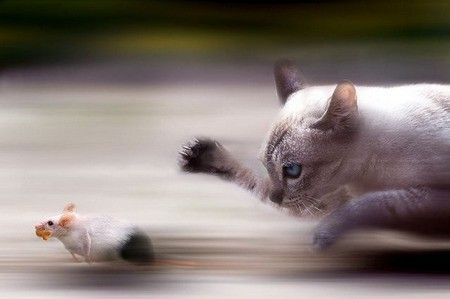
\includegraphics[width=0.4\textwidth]{figs/fast.jpg}
%   \end{center}
%  \end{block}

\end{frame}


\begin{frame}[fragile]
\frametitle{Basic Usage: Data Management}
 \begin{block}{Granularity of Operations}
  \begin{itemize}
   \item Filling a vector with data
   \begin{lstlisting}
viennacl::vector<double> v(10000);

for (size_t i=0; i<v.size(); ++i)
  v(i) = i;    
   \end{lstlisting}
  \end{itemize}
 \end{block}

 \begin{block}{GPU Computing Is Fast, Right?}
  \begin{itemize}
   \item Execution time: 1 sec (approx)
   \item \texttt{std::vector}: $<$ 1 ms
  \end{itemize}

 \end{block}

 \vspace*{2.5cm}

\end{frame}

% \begin{frame}[fragile]
% \frametitle{Basic Usage: Data Management}
%  \begin{block}{Granularity of Operations}
%   \begin{itemize}
%    \item Filling a vector with data
%    \begin{lstlisting}
% viennacl::vector<double> v(10000);
% 
% for (size_t i=0; i<v.size(); ++i)
%   v(i) = i;    
%    \end{lstlisting}
%   \end{itemize}
%  \end{block}
% 
%  \begin{block}{GPU Computing Is Fast, Right?}
%   \begin{center}
%     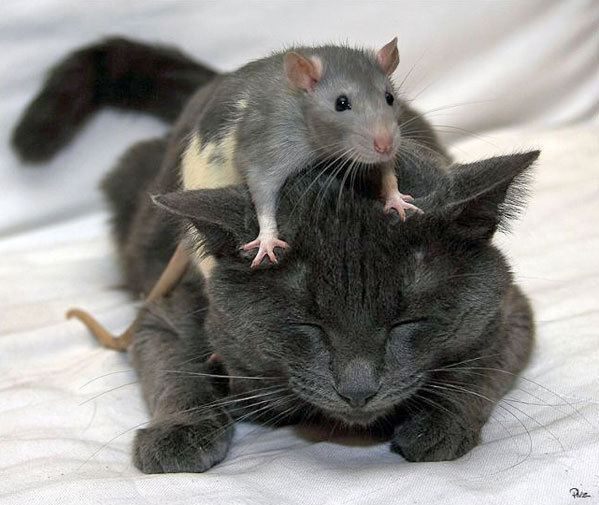
\includegraphics[width=0.35\textwidth]{figs/fast2.jpg}
%   \end{center}
%  \end{block}
% 
% \end{frame}


\begin{frame}[fragile]
\frametitle{Basic Usage: Data Management}
\begin{block}{Granularity of Operations}
 \begin{itemize}
  \item Transfer is done for each element separately
  \item High overhead, similar to scalar operations
 \end{itemize}
\end{block}

\begin{block}{How to avoid the pitfall}
 \begin{itemize}
  \item Use temporary vector
  \item Use copy functions
 \end{itemize}
   \begin{lstlisting}
viennacl::vector<double> v(10000);
std::vector<double> cpu_v( v.size() );

for (size_t i=0; i<cpu_v.size(); ++i)
  cpu_v(i) = i; 

viennacl::copy(cpu_v, v);
   \end{lstlisting}
\end{block}
\end{frame}



\begin{frame}[fragile]
\frametitle{Basic Usage: Data Management}

\begin{block}{How to access/transfer ViennaCL vectors/matrices elements?}
  \begin{itemize}
   \item Direct element access $\Rightarrow$ Bad idea!
   \item Iterator $\Rightarrow$ Bad idea!
   \item Copy functions $\Rightarrow$ \textbf{Good idea!}
  \end{itemize}
  
  \begin{lstlisting}
std::vector<ScalarType> cpu_vec(10);
viennacl::vector<ScalarType> vcl_vec(10);

for (int i = 0; i < 10; ++i)
    cpu_vec[i] = i;
    
viennacl::copy( cpu_vec, vcl_vec );

viennacl::copy( vcl_vec, cpu_vec );
  \end{lstlisting}
\end{block}

\end{frame}



\begin{frame}[fragile]
\frametitle{Basic Usage: Data Management}

\begin{block}{Fast copy}
  \begin{itemize}
   \item copy does not require linear arrays $\Rightarrow$ temporary required
   \item 
  \end{itemize}
  
  \begin{lstlisting}
std::list<ScalarType> cpu_vec(10);
viennacl::vector<ScalarType> vcl_vec(10);

for (int i = 0; i < 10; ++i)
    cpu_vec[i] = i;
    
viennacl::copy( cpu_vec, vcl_vec );

viennacl::copy( vcl_vec, cpu_vec );
  \end{lstlisting}
\end{block}

\end{frame}



\begin{frame}[fragile]
\frametitle{Basic Usage: Data Management}

\begin{block}{Fast copy}
  \begin{itemize}
   \item copy does not require linear arrays $\Rightarrow$ temporary required
   \item If container is linear memory $\Rightarrow$ use fast\_copy instead
  \end{itemize}
  
  \begin{lstlisting}
std::|\color{red}vector|<ScalarType> cpu_vec(10);
viennacl::vector<ScalarType> vcl_vec(10);

for (int i = 0; i < 10; ++i)
    cpu_vec[i] = i;
    
|\color{red}viennacl::fast\_copy( cpu\_vec, vcl\_vec );|

|\color{red}viennacl::fast\_copy( vcl\_vec, cpu\_vec );|
  \end{lstlisting}
\end{block}

\end{frame}




\begin{frame}
\frametitle{Basic Usage: Algebra}

\begin{block}{Algebra operations}
  \begin{itemize}
   \item Trivial operations done by \textbf{operator overloading}
   \item Scalar multiplication support for vector and matrices
   \item Inner product and norm support for vectors
   \item Matrix transpose using function \textbf{trans}
   \item Matrix-vector and matrix-matrix multiplication using function \textbf{prod}
  \end{itemize}
\end{block}

\end{frame}



\begin{frame}[fragile]
\frametitle{Basic Usage: Algebra}

\begin{block}{Scalar operations}
  \begin{lstlisting}
NumericType s1, s2;
viennacl::scalar<NumericType> vcl_s1, vcl_s2, vcl_s3;

vcl_s1  = 5;
vcl_s2  = vcl_s1 * 3;
vcl_s3 -= vcl_s1 + (vcl_s2 / 4);

s1      = vcl_s3;
s2      = vcl_s1 - vcl_s2 * 2;
  \end{lstlisting}
\end{block}

\end{frame}



\begin{frame}[fragile]
\frametitle{Basic Usage: Algebra}

\begin{block}{Vector operations}
  \begin{lstlisting}
viennacl::scalar<NumericType> vcl_s1, vcl_s2;
viennacl::vector<NumericType> v1(10), v2(10), v3(10);

v2  = vcl_s1 * v1 + v2
v3 += vcl_s1 * v2;

v3  = 0.5 * v2 - v3;
  \end{lstlisting}
\end{block}

\end{frame}



\begin{frame}[fragile]
\frametitle{Basic Usage: Algebra}

\begin{block}{Vector operations}
  \begin{lstlisting}
NumericType s1, s2;
viennacl::scalar<NumericType> vcl_s1, vcl_s2;
viennacl::vector<NumericType> v10), v2(10), v3(10);

vcl_s1 = viennacl::linalg::inner_prod(v1, v2);
s1     = viennacl::linalg::inner_prod(v1, v2);
 
s1     = viennacl::linalg::norm_1(v1);
vcl_s2 = viennacl::linalg::norm_2(v2);
s2     = viennacl::linalg::norm_inf(v3);
  \end{lstlisting}
\end{block}

\end{frame}



\begin{frame}[fragile]
\frametitle{Basic Usage: Algebra}

\begin{block}{Matrix operations}
  \begin{lstlisting}
viennacl::scalar<NumericType> vcl_s1, vcl_s2;
viennacl::matrix<NumericType> M1(10, 10),
    M2(10, 10), M3(10,10);

M2  = vcl_s1 * M1 + M2
M3 += vcl_s2 * M2;

M3  = 0.5 * M2 -  M3;

M3  = viennacl::trans(M2); // Transposed matrix

// Matrix-matrix product
M1  = viennacl::linalg::prod( M2, M3 );
M1  = viennacl::linalg::prod( M2, viennacl::trans(M3) );
  \end{lstlisting}
\end{block}

\end{frame}


\begin{frame}[fragile]
\frametitle{Basic Usage: Algebra}

\begin{block}{GEMM: ViennaCL vs. CUBLAS}
  \begin{lstlisting}
// ViennaCL
M1 = vcl_s1 * prod( M2, trans(M3) ) + vcl_s2 * M3;

// CUBLAS
cublasStatus_t cublasDgemm(handle,
    transa, transb,
    m, n, k,
    alpha,
    A, lda,
    B, ldb,
    beta,
    C, ldc);
  \end{lstlisting}
\end{block}

\end{frame}




\begin{frame}[fragile]
\frametitle{Basic Usage: Algebra}

\begin{block}{Matrix-vector operations}
  \begin{lstlisting}
viennacl::vector<NumericType> v1(10), v210), v3(20);
viennacl::matrix<NumericType> M1(10, 10), M2(20, 10);

v1 = viennacl::linalg::prod( M1, v2 );
v1 = viennacl::linalg::prod( viennagrid::trans(M1), v2 );
v3 = viennacl::linalg::prod( M2, v2 );
v1 = viennacl::linalg::prod( M1, v3 );
    // ERROR! dimension missmatch
  \end{lstlisting}
\end{block}

\end{frame}



\begin{frame}
\frametitle{Basic Usage: Solver}

\begin{block}{Solving a system of linear equations}
  \begin{itemize}
   \item $Ax=b$
   \item A and b given, x is unknown
   \item Common problem in mathematics
  \end{itemize}
\end{block}

\begin{block}{Types of solver}
  \begin{itemize}
   \item Direct solver
   \item Iterative solver
  \end{itemize}
\end{block}

\end{frame}



\begin{frame}
\frametitle{Basic Usage: Solver}

\begin{block}{Direct solver}
  \begin{itemize}
   \item Solving the system directly
   \item e.g. Gaussian elimination with pivoting
  \end{itemize}
\end{block}

\begin{block}{Iterative solver}
  \begin{itemize}
   \item Solving using an iterative process
   \item Convergence relies on matrix properties
   \item Recommended for large and sparse systems
   \item No write operation needed on matrix\\(most only use matrix-vector multiplication)
  \end{itemize}
\end{block}

\end{frame}



\begin{frame}[fragile]
\frametitle{Basic Usage: Solver}

\begin{block}{Direct solver}
  \begin{itemize}
   \item LU factorization
   \item No pivoting (work in progress)
  \end{itemize}
  
  \begin{lstlisting}
using namespace viennacl::linalg;

viennacl::matrix<float> vcl_matrix;
viennacl::vector<float> vcl_rhs, vcl_result;
/* Set up matrix and vectors here */

//solution of an upper triangular system:
vcl_result = solve(vcl_matrix, vcl_rhs, upper_tag());
//solution of a lower triangular system:
vcl_result = solve(vcl_matrix, vcl_rhs, lower_tag());

//solution of a full system right into the vector vcl_rhs:
lu_factorize(vcl_matrix);
lu_substitute(vcl_matrix, vcl_rhs);
  \end{lstlisting}
\end{block}

\end{frame}


\begin{frame}
\frametitle{Basic Usage: Solver}

\begin{block}{Iterative solver}
  \begin{itemize}
   \item Conjugate Gradient (CG)
   \item Stabilized Bi-CG (BiCGStab)
   \item Generalized Minimum Residual (GMRES)
  \end{itemize}
\end{block}

\begin{table}[tb]
\begin{center}
\scriptsize
\renewcommand{\arraystretch}{1.2}
\begin{tabular}{p{2.5cm}|p{1.5cm}|p{5cm}}
Method & Matrix class & ViennaCL\\
\hline
\hline
Conjugate Gradient (CG) & symmetric positive definite & \texttt{y = solve(A, x, cg\_tag());} \\
\hline
Stabilized Bi-CG (BiCGStab) & non-symmetric & \texttt{y = solve(A, x, bicgstab\_tag());} \\
\hline
Generalized Minimum Residual (GMRES) & general & \texttt{y = solve(A, x, gmres\_tag());} \\
\hline
\hline
\end{tabular}
\end{center}
\end{table}

\end{frame}



\begin{frame}[fragile]
\frametitle{Basic Usage: Solver}

\begin{block}{Iterative solver}
  \begin{itemize}
   \item Solver configuration via tag
  \end{itemize}
  
  \begin{lstlisting}
using namespace viennacl::linalg;

// conjugate gradient solver with tolerance 1e10
// and at most 100 iterations:
viennacl::linalg::cg_tag custom_cg(1e-10, 100);

vcl_result = solve(vcl_matrix, vcl_rhs, custom_cg);

//print number of iterations taken and estimated error:
cout << "No. of iters: " << custom_cg.iters() << endl;
cout << "Est. error: " << custom_cg.error() << endl;
  \end{lstlisting}
\end{block}

\end{frame}



\begin{frame}{Summary}
\begin{block}{What have we learned?}
  \begin{itemize}
   \item ViennaCL provides interface compatibility with Boost.uBLAS
   \item Basic types of ViennaCL
   \item How OpenCL kernels are used
   \item How to transfer data to and from ViennaCL
   \item How to work with ViennaCL types
   \item Simple algebraic operations
   \item Solver for systems of linear equations
  \end{itemize}
\end{block}
\end{frame}



% \begin{frame}{Summary}
% \TODO{Achievment unlocked: ViennaCL apprentice}
% \end{frame}
% 
% 
% \begin{frame}{Summary}
% \TODO{Einleitung in die Pause}
% \end{frame}

% Advanced ViennaCL

\begin{frame}{ }
 \begin{center}
  \Large \textbf{How-To: Advanced \ViennaCL}
 \end{center}
\end{frame}


\begin{frame}{How-To: Advanced \ViennaCL}

\begin{block}{What to expect}
  \begin{itemize}
   \item Subvectors and Submatrices
   \item Escaping the Curse of Temporaries
   \item Interface: Eigen
   \item Performance
   \item Summary
  \end{itemize}
\end{block}

\end{frame}



\begin{frame}[fragile]
\frametitle{Subvectors and Submatrices}
 \begin{block}{Important for Many Algorithms}
  \begin{itemize}
   \item LU, Cholesky
   \item QR, SVD
  \end{itemize}
 \end{block}

 \begin{block}{Two sub-types available}
  \begin{itemize}
   \item Range $[a,b)$
   \item Slice $a$:inc:size
  \end{itemize}
 \end{block}

 \begin{block}{Ranges and slices are proxies}
  \begin{itemize}
   \item Read- and writeable
  \end{itemize}
 \end{block}
 
\end{frame}



\begin{frame}[fragile]
\frametitle{Subvectors and Submatrices}

  \begin{block}{Range example}
 \begin{lstlisting}
std::size_t lower_bound = 1;
std::size_t upper_bound = 7;
viennacl::range r(lower_bound, upper_bound);

typedef viennacl::vector<ScalarType> VectorType;
typedef viennacl::matrix<ScalarType> MatrixType;

// v[1:6]
viennacl::vector_range<VCLVectorType> v_sub(v, r);
// M[1:6,1:6]
viennacl::matrix_range<VCLMatrixType> M_sub(M, r, r);
 \end{lstlisting}
 \end{block}

 \vspace{0.45cm}
 
\end{frame}



\begin{frame}[fragile]
\frametitle{Subvectors and Submatrices}

\begin{block}{Slice example}
 \begin{lstlisting}
std::size_t start = 2;
std::size_t stride = 3;
std::size_t size = 5
viennacl::slice s(start, stride, size);

typedef viennacl::vector<ScalarType> VectorType;
typedef viennacl::matrix<ScalarType> MatrixType;

// v[2, 5, 8, 11, 14]
viennacl::vector_slice<VCLVectorType> v_sub(v, r);
// M[2,2], ..., M[2,14], ..., M[14,2], ..., M[14,14]
viennacl::matrix_slice<VCLMatrixType> M_sub(M, r, r);
 \end{lstlisting}
 \end{block}

\end{frame}



\begin{frame}[fragile]
\frametitle{Subvectors and Submatrices}
 \begin{block}{Convenience Functions}
 \begin{lstlisting}
viennacl::vector<ScalarType> v1(4), v2(2);
viennacl::matrix<ScalarType> M1(4,4), M2(2,2);
 
range r(0, 2);
slice s(0, 2, 2);

v2 = project(v1, r);
project(v1, s) = v2;

M2 = project(M1, r, r);
viennacl::copy(M2, project(M1, s, s) );
 \end{lstlisting}
 \end{block}

\end{frame}



\begin{frame}[fragile]
\frametitle{Subvectors and Submatrices}
 \begin{block}{Copy Headaches: Row-Major}
   \begin{center}
     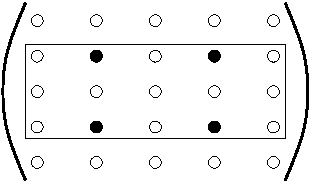
\includegraphics[width=0.35\textwidth]{figs/copy-matrix-row-coarse.pdf} \hspace*{0.5cm}
     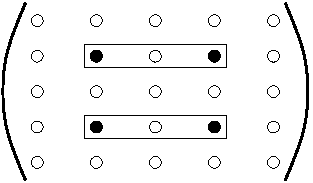
\includegraphics[width=0.35\textwidth]{figs/copy-matrix-row-fine.pdf}
   \end{center}
 \end{block}

 \begin{block}{Copy Headaches: Column-Major}
   \begin{center}
     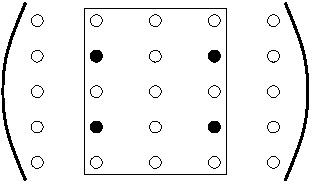
\includegraphics[width=0.35\textwidth]{figs/copy-matrix-col-coarse.pdf} \hspace*{0.5cm}
     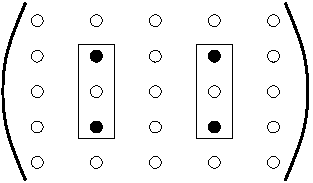
\includegraphics[width=0.35\textwidth]{figs/copy-matrix-col-fine.pdf}
   \end{center}
 \end{block}

\end{frame}





\begin{frame}[fragile]
\frametitle{Escaping the Curse of Temporaries}

 \begin{block}{Simple BLAS Level 1 Operation}
  \begin{itemize}
   \item Consider
  {\black \begin{lstlisting}
 vec1 = vec2 + alpha * vec3 - beta * vec4;
  \end{lstlisting} }

    \item  With naive C++, this is equivalent to
  {\black \begin{lstlisting}
tmp1 <- alpha * vec3
tmp2 <- beta * vec4;
tmp3 <- tmp1 - tmp2;
tmp4 <- vec2 + tmp3;
vec1 <- tmp4;
  \end{lstlisting} }
  \end{itemize}
  
 \end{block}

  \begin{block}{Temporaries Lead to Poor Performance}
    \begin{itemize}
     \item Costly on CPUs, extremely expensive on GPUs
     \item Use expression templates for avoiding temporaries
    \end{itemize}
  \end{block}
  
\vspace*{0.3cm}
\end{frame}




\begin{frame}[fragile]
\frametitle{Escaping the Curse of Temporaries}

 \begin{block}{Vector Addition}
  \begin{lstlisting}
 x = y + z;
  \end{lstlisting}
 \end{block}

  %\pause

 \begin{block}{Naive Operator Overloading}
  \begin{lstlisting}
 vector<T> operator+(vector<T> & v, vector<T> & w);
  \end{lstlisting}

  %\pause

  \begin{itemize}
   \item t $\leftarrow$ y + z, x $\leftarrow$ t
   %\pause
   \item Temporaries are extremely expensive! 
  \end{itemize}
 \end{block}

   %\pause



\end{frame}



\begin{frame}[fragile]
\frametitle{Escaping the Curse of Temporaries}
 \begin{block}{Expression Templates}
  \begin{lstlisting}
 vector_expr<vector<T>, op_plus, vector<T> >
 operator+(vector<T> & v, vector<T> & w) { ... }

 vector::operator=(vector_expr<...> const & e) {
   viennacl::linalg::avbv(*this, 1,e.lhs(), 1,e.rhs());
 }
  \end{lstlisting}
  \vspace*{0.5cm}

 \end{block}

%  \begin{block}{\texttt{vector\_expression} does not compute anything}
%    \begin{itemize}
%     \item Represents the expression only
%    \end{itemize}
%  \end{block}

  \begin{block}{Allows to Avoid a Significant Amount of Temporaries}
    \begin{itemize}
     \item Covers most frequent cases
     \item Influence on compilation times moderate
    \end{itemize}
  \end{block}
\end{frame}



\begin{frame}[fragile]
\frametitle{Escaping the Curse of Temporaries}
  \begin{block}{Expression templates have their limitations}
  \begin{lstlisting}
viennacl::vector<NumericType> v;
viennacl::matrix<NumericType> M;

v = viennacl::linalg::prod(M, v);
  \end{lstlisting}
  
    \begin{itemize}
     \item Temporary object is required here!
     \item ViennaCL detects such cases and takes care of it
    \end{itemize}
 \end{block}

\end{frame}



\begin{frame}{Interface: Eigen}
\begin{block}{Data transfer}
 \begin{itemize}
  \item Like transfer from and to std container
  \item Using provided copy functions
 \end{itemize}
\end{block}

\begin{block}{Interface compatibility}
 \begin{itemize}
  \item ViennaCL algorithms work with Eigen
  \item e.g.: iterative solver
 \end{itemize}
\end{block}
\end{frame}



\begin{frame}[fragile]
\frametitle{Interface: Eigen}
\begin{block}{Data transfer: vectors}
  \begin{lstlisting}
#define VIENNACL_HAVE_EIGEN
 
Eigen::VectorXd eigen_vector(dim);
 
// fill Eigen objects in a very sophisticated way with numbers here
 
viennacl::vector<double> viennacl_vector(dim);
 
// copy data from Eigen objects to ViennaCL objects
viennacl::copy(eigen_vector, viennacl_vector);
 
// do some heavy linear algebra with ViennaCL here 
 
// copy back to Eigen:
viennacl::copy(viennacl_vector, eigen_vector);
  \end{lstlisting} 
\end{block}

\end{frame}



\begin{frame}[fragile]
\frametitle{Interface: Eigen}
\begin{block}{Data transfer: dense matrix}
  \begin{lstlisting}
#define VIENNACL_HAVE_EIGEN
 
Eigen::MatrixXd eigen_densematrix(dim, dim);
 
// fill Eigen objects in a very sophisticated way with numbers here
 
viennacl::matrix<double> viennacl_densematrix(dim, dim);
 
// copy data from Eigen objects to ViennaCL objects
viennacl::copy(eigen_densematrix,viennacl_densematrix);
 
// do some heavy linear algebra with ViennaCL here 
 
// copy back to Eigen:
viennacl::copy(viennacl_densematrix, eigen_densematrix);
  \end{lstlisting} 
\end{block}

\end{frame}



\begin{frame}[fragile]
\frametitle{Interface: Eigen}
\begin{block}{Data transfer: sparse matrix}
  \begin{lstlisting}
#define VIENNACL_HAVE_EIGEN
 
Eigen::SparseMatrix<double, Eigen::RowMajor> eigen_sparsematrix(dim, dim);
 
// fill Eigen objects in a very sophisticated way with numbers here
 
viennacl::compressed_matrix<double> viennacl_sparsematrix(dim, dim);
 
// copy data from Eigen objects to ViennaCL objects
viennacl::copy(eigen_sparsematrix, viennacl_sparsematrix);
 
// do some heavy linear algebra with ViennaCL here 
 
// copy back to Eigen:
viennacl::copy(viennacl_sparsematrix, eigen_sparsematrix);
  \end{lstlisting} 
\end{block}

\end{frame}



\begin{frame}[fragile]
\frametitle{Interface: Eigen}
\begin{block}{Interface Compatibility: iterative solver}
  \begin{lstlisting}
#define VIENNACL_HAVE_EIGEN
using namespace viennacl::linalg;
 
Eigen::SparseMatrix<double, Eigen::RowMajor>
    matrix(dim, dim);
Eigen::VectorXd rhs(dim);
Eigen::VectorXd result(dim);
// fill eigen_matrix and eigen_rhs here
 
// Solve system using CG from ViennaCL
result = solve(matrix, rhs, cg_tag());
 
// Solve system using BiCGStab from ViennaCL
result = solve(matrix, rhs, bicgstab_tag());
 
// Solve system using GMRES from ViennaCL
result = solve(matrix, rhs, gmres_tag());
  \end{lstlisting} 
\end{block}

\end{frame}






%%%%%%%

\begin{frame}[fragile]
\frametitle{Performance}
 \begin{block}{Granularity of Operations}
  \begin{itemize}
   \item Solving linear systems
   \begin{lstlisting}
viennacl::matrix<double> mat(N, N);
viennacl::vector<double> rhs(N);

for (size_t i=0; i<1000; ++i)
{
   viennacl::vector<double> result 
     = solve(mat, rhs, bicgstab_tag());
   /* process result */
}
   \end{lstlisting}
  \end{itemize}
 \end{block}

 \begin{block}{Why Is There No Speed-Up?}
   \begin{itemize}
    \item 
   \end{itemize}
 \end{block}

\end{frame}


\begin{frame}[fragile]
\frametitle{Performance}
 \begin{block}{Granularity of Operations}
  \begin{itemize}
   \item Solving linear systems
   \begin{lstlisting}
viennacl::matrix<double> mat(N, N);
viennacl::vector<double> rhs(N);

for (size_t i=0; i<1000; ++i)
{
   viennacl::vector<double> result 
     = solve(mat, rhs, bicgstab_tag());
   /* process result */
}
   \end{lstlisting}
  \end{itemize}
 \end{block}

 \begin{block}{Why Is There No Speed-Up?}
   \begin{itemize}
    \item $N = 3$
   \end{itemize}
 \end{block}

\end{frame}


\begin{frame}[fragile]
\frametitle{Performance}

Lets take a look

\end{frame}



\begin{frame}[fragile]
\frametitle{Performance}
 \begin{block}{Sample Operation}
  \begin{itemize}
   \item $v_1 \leftarrow v_2$
  \end{itemize}

   \begin{center}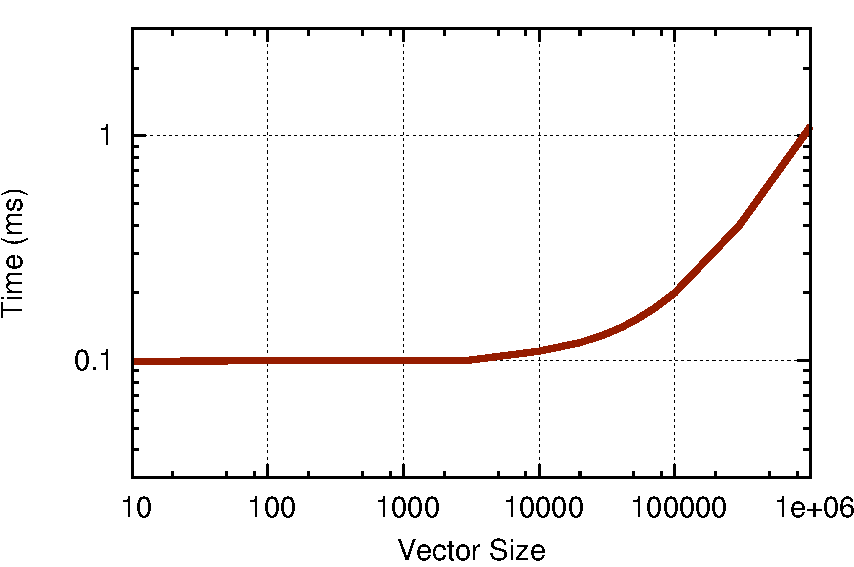
\includegraphics[width=0.6\textwidth]{figs/kernel-launch.pdf} \end{center}
 \end{block}

 \begin{block}{OpenCL Kernel Launch Overhead}
   \begin{itemize}
    \item $10-100$ $\mu$s
   \end{itemize}
 \end{block}

\end{frame}



\begin{frame}[fragile]
\frametitle{Performance}
 \begin{block}{GPUs: Disillusion - Computing Architecture Schematic}
  \begin{center}
   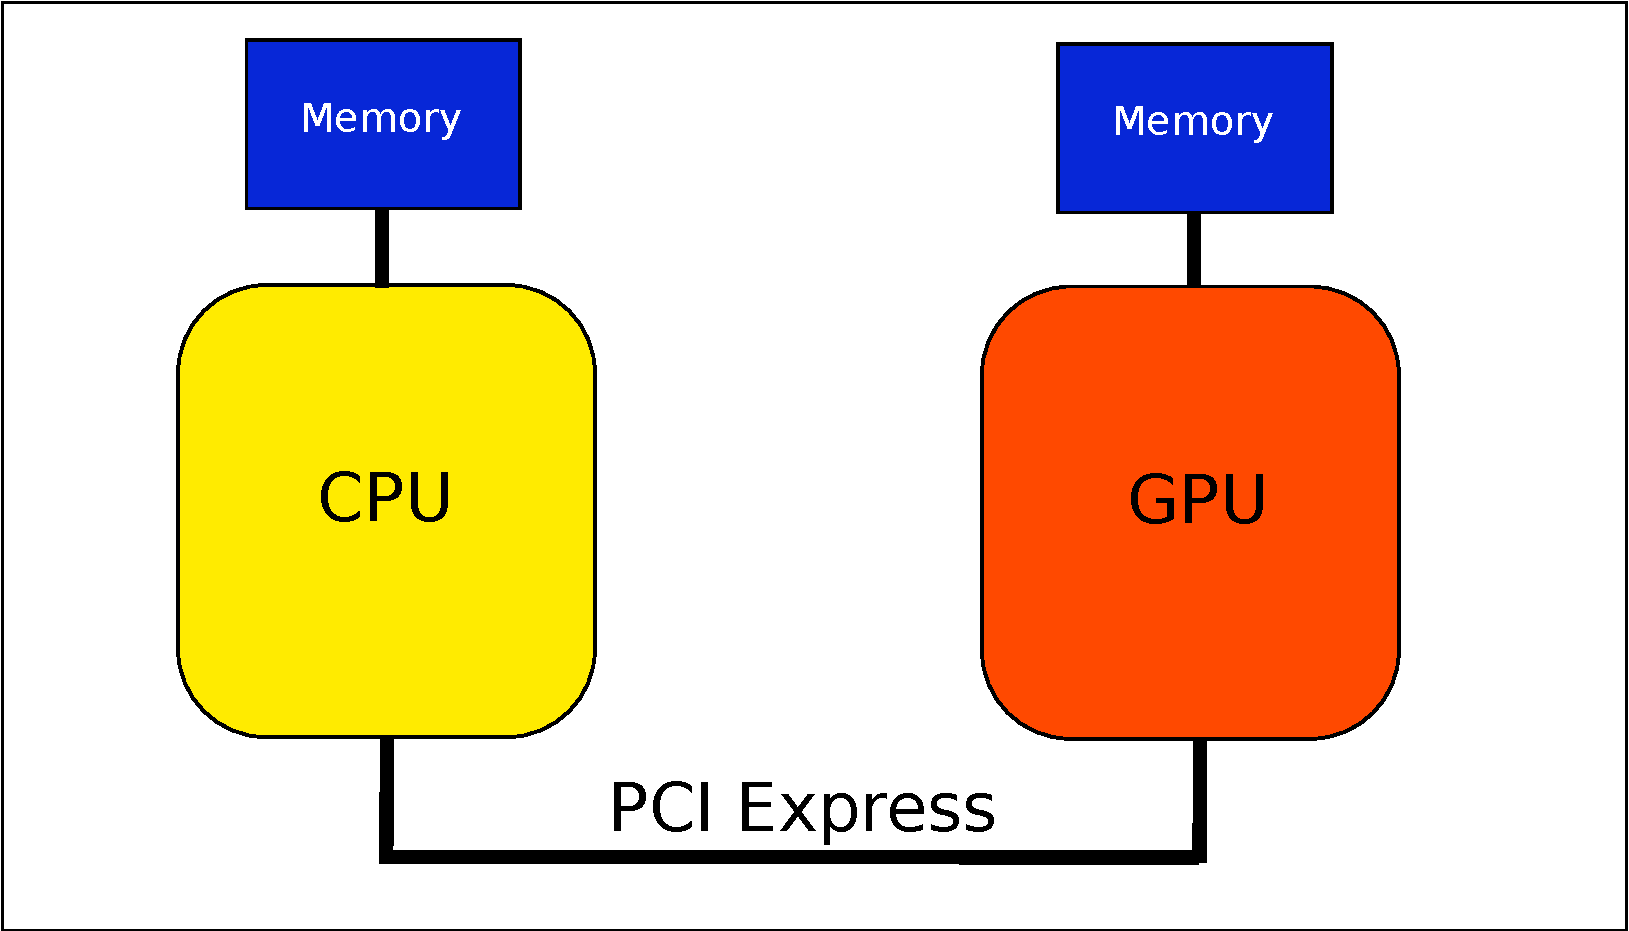
\includegraphics[width=0.7\textwidth]{figs/cpu-gpu-coarse.pdf}
  \end{center}

 
 \begin{itemize}
  \item \vspace*{1.12cm}
 \end{itemize}
 \end{block}

\end{frame}

\begin{frame}[fragile]
\frametitle{Performance}
 \begin{block}{GPUs: Disillusion - Computing Architecture Schematic}
  \begin{center}
   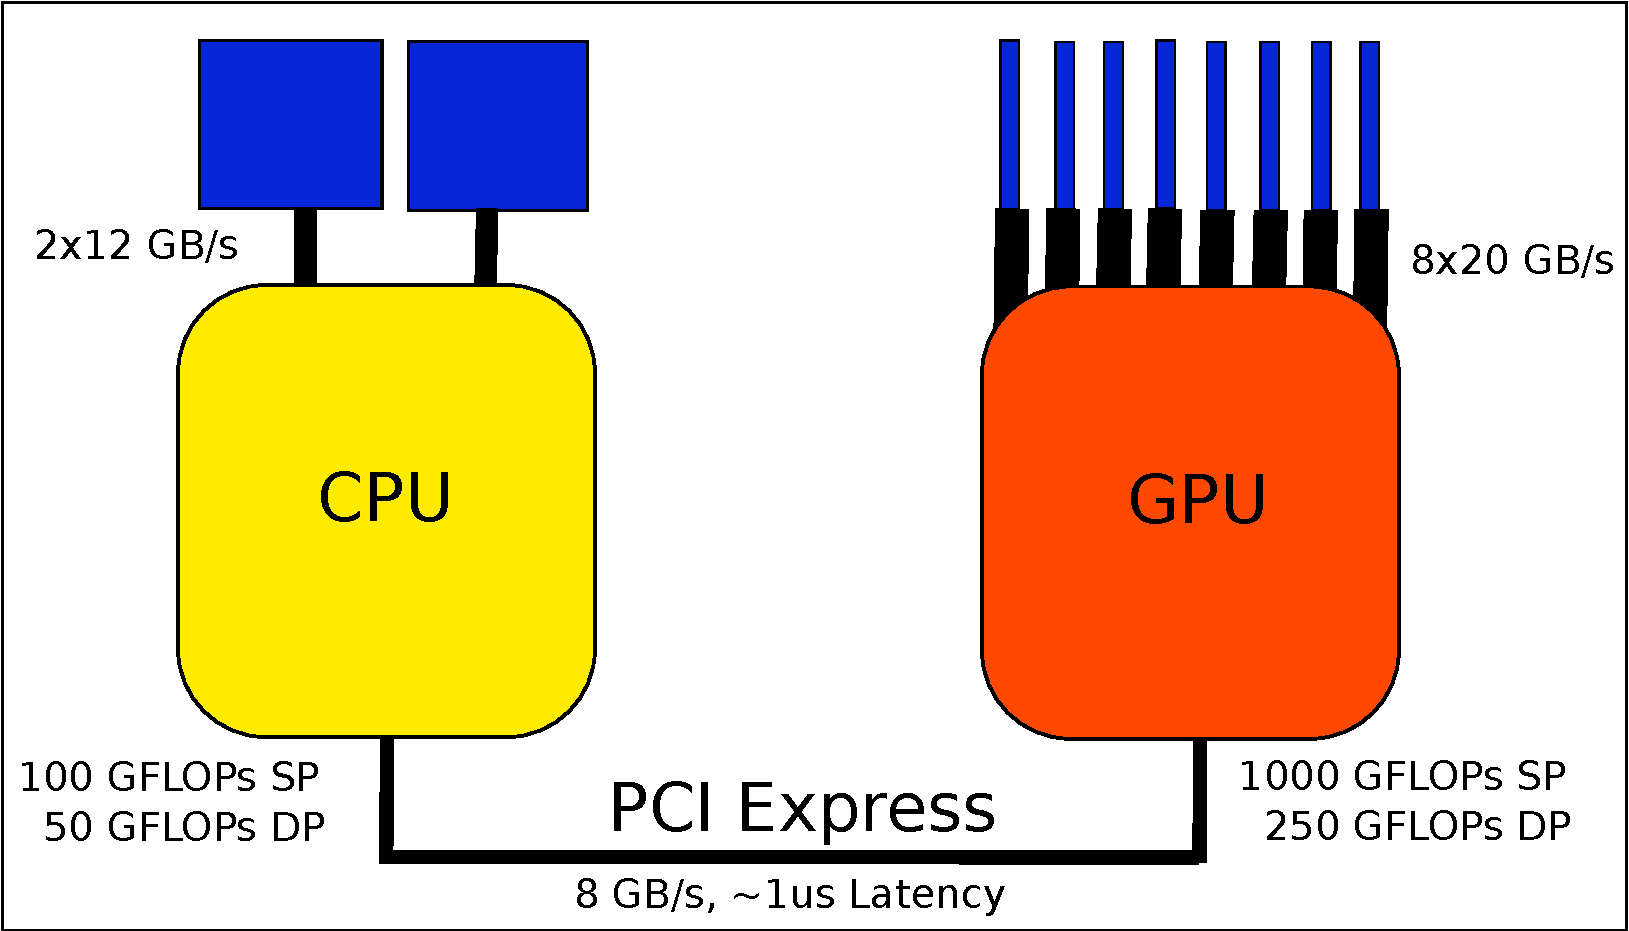
\includegraphics[width=0.7\textwidth]{figs/cpu-gpu-detail.pdf}
  \end{center}

 \begin{itemize}
  \item Good for large FLOP-intensive tasks, high memory bandwidth
  \item PCI-Express can be a bottleneck
  \item $\gg 10$-fold speedups (usually) not backed by hardware
 \end{itemize}
 \end{block}

\end{frame}



\begin{frame}{Performance}
\begin{block}{Some benchmarks - vector addition}
  \begin{center}
   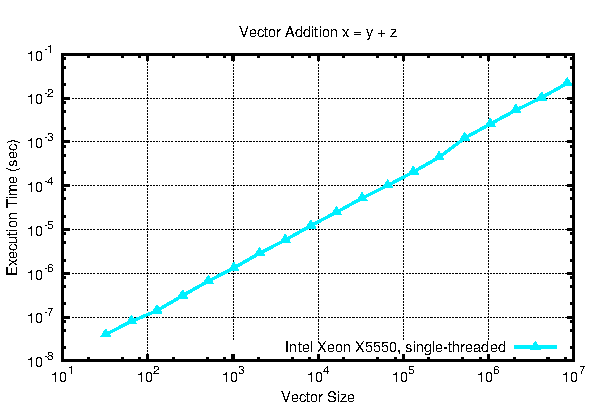
\includegraphics[width=0.9\textwidth]{figs/vector-timings-1}
  \end{center}
\end{block}
\end{frame}

\begin{frame}{Performance}
\begin{block}{Some benchmarks - vector addition}
  \begin{center}
   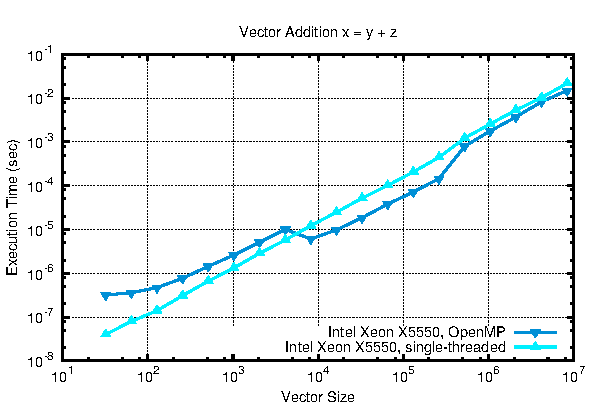
\includegraphics[width=0.9\textwidth]{figs/vector-timings-2}
  \end{center}
\end{block}
\end{frame}

\begin{frame}{Performance}
\begin{block}{Some benchmarks - vector addition}
  \begin{center}
   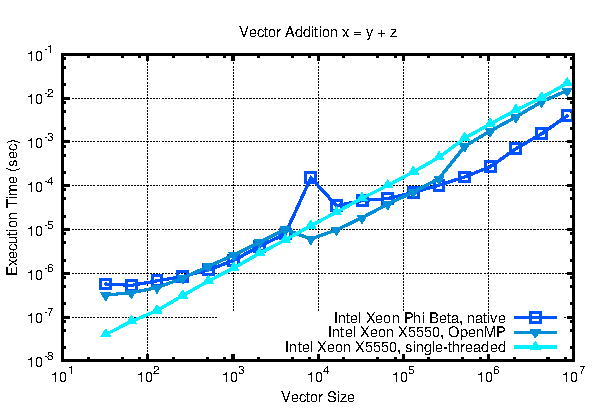
\includegraphics[width=0.9\textwidth]{figs/vector-timings-3}
  \end{center}
\end{block}
\end{frame}

\begin{frame}{Performance}
\begin{block}{Some benchmarks - vector addition}
  \begin{center}
   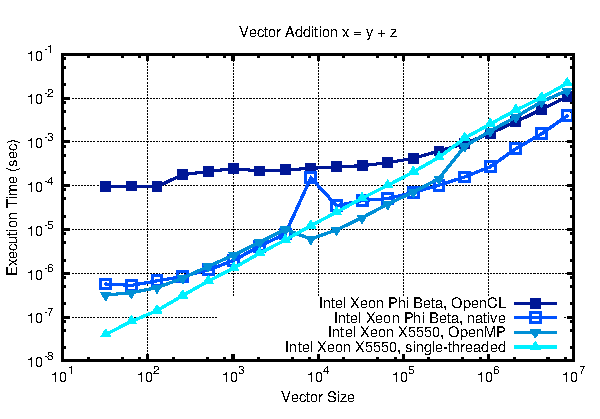
\includegraphics[width=0.9\textwidth]{figs/vector-timings-4}
  \end{center}
\end{block}
\end{frame}

\begin{frame}{Performance}
\begin{block}{Some benchmarks - vector addition}
  \begin{center}
   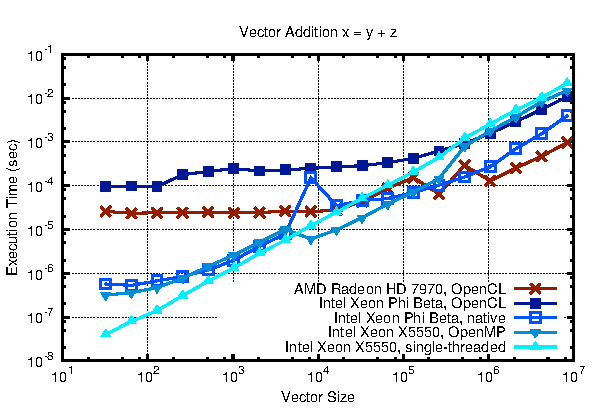
\includegraphics[width=0.9\textwidth]{figs/vector-timings-5}
  \end{center}
\end{block}
\end{frame}

\begin{frame}{Performance}
\begin{block}{Some benchmarks - vector addition}
  \begin{center}
   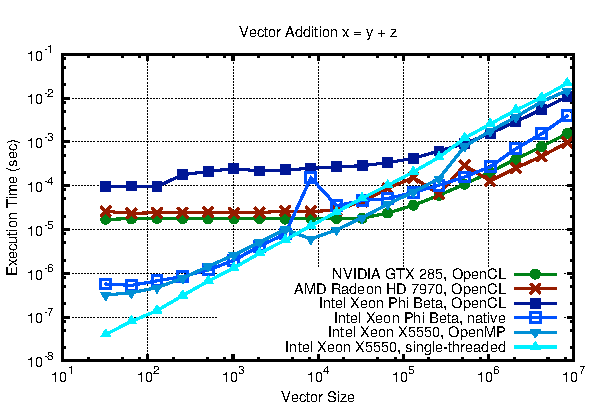
\includegraphics[width=0.9\textwidth]{figs/vector-timings-6}
  \end{center}
\end{block}
\end{frame}

\begin{frame}{Performance}
\begin{block}{Some benchmarks - vector addition}
  \begin{center}
   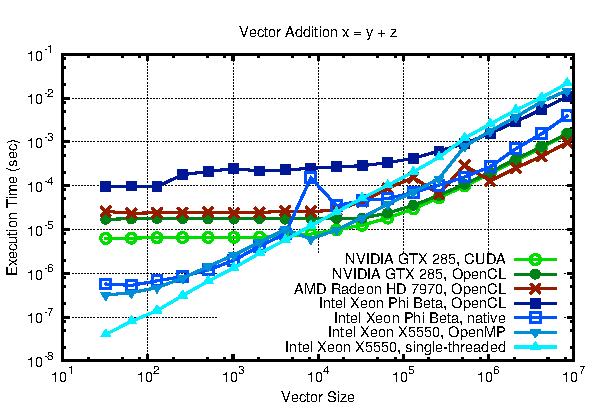
\includegraphics[width=0.9\textwidth]{figs/vector-timings-7}
  \end{center}
\end{block}
\end{frame}



\begin{frame}{Performance}
\begin{block}{Some benchmarks - CG solver}
  \begin{center}
   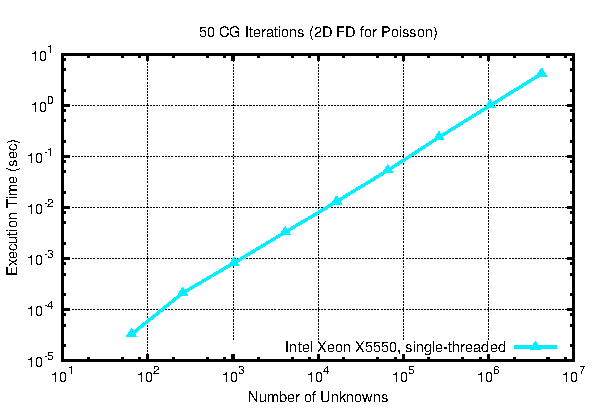
\includegraphics[width=0.9\textwidth]{figs/cg-timings-1}
  \end{center}
\end{block}
\end{frame}

\begin{frame}{Performance}
\begin{block}{Some benchmarks - CG solver}
  \begin{center}
   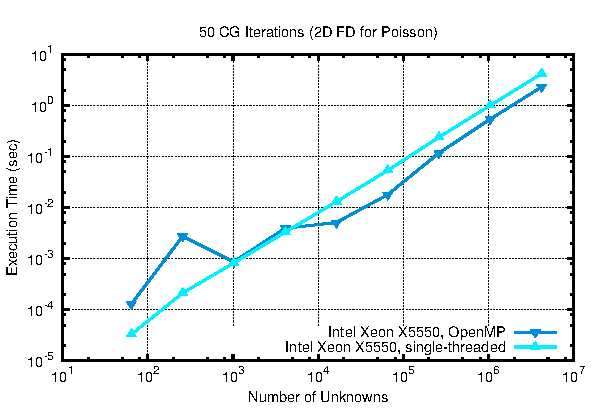
\includegraphics[width=0.9\textwidth]{figs/cg-timings-2}
  \end{center}
\end{block}
\end{frame}

\begin{frame}{Performance}
\begin{block}{Some benchmarks - CG solver}
  \begin{center}
   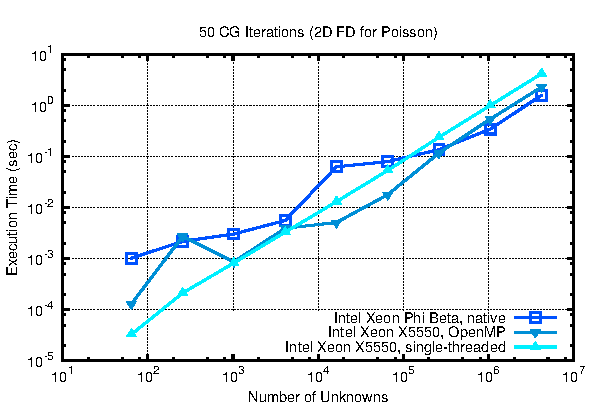
\includegraphics[width=0.9\textwidth]{figs/cg-timings-3}
  \end{center}
\end{block}
\end{frame}

\begin{frame}{Performance}
\begin{block}{Some benchmarks - CG solver}
  \begin{center}
   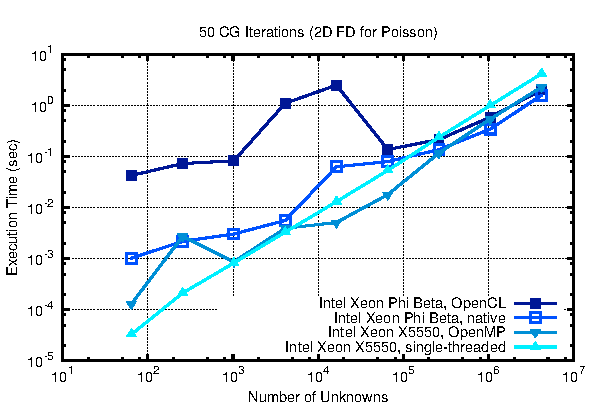
\includegraphics[width=0.9\textwidth]{figs/cg-timings-4}
  \end{center}
\end{block}
\end{frame}

\begin{frame}{Performance}
\begin{block}{Some benchmarks - CG solver}
  \begin{center}
   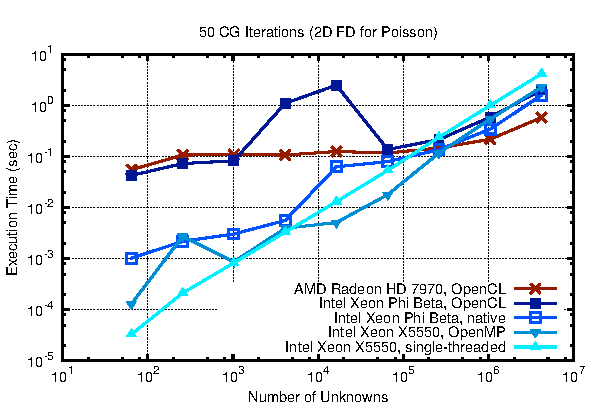
\includegraphics[width=0.9\textwidth]{figs/cg-timings-5}
  \end{center}
\end{block}
\end{frame}

\begin{frame}{Performance}
\begin{block}{Some benchmarks - CG solver}
  \begin{center}
   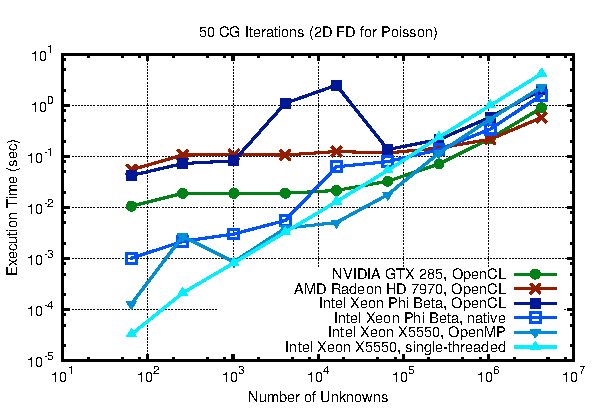
\includegraphics[width=0.9\textwidth]{figs/cg-timings-6}
  \end{center}
\end{block}
\end{frame}

\begin{frame}{Performance}
\begin{block}{Some benchmarks - CG solver}
  \begin{center}
   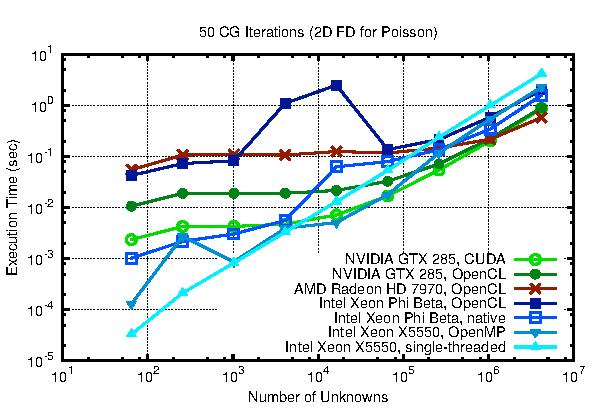
\includegraphics[width=0.9\textwidth]{figs/cg-timings-7}
  \end{center}
\end{block}
\end{frame}



\begin{frame}{Performance}
 \begin{block}{Some benchmarks - Matrix-Matrix Multiplication}
  \begin{itemize}
   \item Auto-tuning environment  (AMD Radeon HD 7970, single precision)
   \item 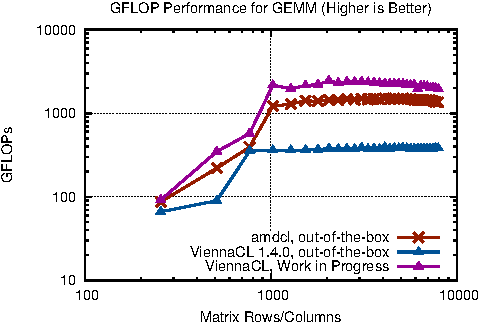
\includegraphics[width=0.85\textwidth]{figs/gemm3.pdf}
  \end{itemize}
 \end{block}
\end{frame}





\begin{frame}{Summary}
\begin{block}{What have we learned?}
  \begin{itemize}
   \item What are subvectors/submatrices and how to use them
   \item How to eliminate temporaries
   \item Expression templates and when they help us
   \item Interface to Eigen
   \item ViennaCL isn't optimized for small vectors/matrices
   \item Performance bottleneck
   \item Overview of ViennaCL performance
  \end{itemize}
\end{block}
\end{frame}


% \begin{frame}{Summary}
% \TODO{Achievement unlocked: ViennaCL expert}
% \end{frame}


















% ViennaCL: behind the curtain

\begin{frame}{ }
 \begin{center}
  \Large \textbf{\ViennaCL : Behind the curtain}
 \end{center}
\end{frame}


\begin{frame}{\ViennaCL : Behind the curtain}

\begin{block}{What to expect}
  \begin{itemize}
   \item Backends
   \item OpenCL kernel management
   \item Extending ViennaCL
   \item ViennaCL and OpenGL
   \item Summary
  \end{itemize}
\end{block}

\end{frame}



\begin{frame}{\ViennaCL : Behind the curtain}

\begin{block}{Backends}
  \begin{itemize}
   \item There is more than OpenCL
   \item CUDA from NVIDIA
   \item OpenACC
   \item Each framework has advantages and disadvantages
  \end{itemize}
\end{block}

\end{frame}



\begin{frame}[fragile]
\frametitle{Backends}
 \begin{block}{OpenCL}
  { \lstset{ basicstyle=\scriptsize\ttfamily } \begin{lstlisting}
const char *kernel_string =
"__kernel void mykernel(__global double *buffer) {
  buffer[get_global_id(0)] = 42.0;
};";   

int main() {
  ...
  cl_program my_prog = clCreateProgramWithSource(
         my_context,1,&kernel_string,&source_len,&err);
  clBuildProgram(my_prog,0,NULL,NULL,NULL,NULL);
  cl_kernel my_kernel = clCreateKernel(my_prog,
                          "mykernel",&err);
  clSetKernelArg(my_kernel,0,sizeof(cl_mem),&buffer);
  clEnqueueNDRangeKernel(queue,my_kernel,1,NULL,
               &global_size,&local_size,0,NULL,NULL);
} 
  \end{lstlisting} }

  \begin{itemize}
   \item Additional boilerplate code required (low-level API)
   \item Broad hardware support (separate SDKs)
   \item No more development effort from NVIDIA
  \end{itemize}
 \end{block}

\end{frame}



\begin{frame}[fragile]
\frametitle{Backends}
 \begin{block}{NVIDIA CUDA}
  { \lstset{ basicstyle=\scriptsize\ttfamily } \begin{lstlisting}
// GPU kernel:
__global__ void kernel(double *buffer)
{
  int idx = blockIdx.x * blockDim.x + threadIdx.x;
  buffer[idx] = 42.0;
}

// host code:
int main()
{ 
  ...
  cudaMalloc((void**)&buffer,size);
  kernel<<<blocknum, blockdim>>>(buffer);
  ...
}
  \end{lstlisting} }

  \begin{itemize}
   \item Almost no additional code required
   \item Vendor-lock
   \item Relies on \lstinline|nvcc| being available
  \end{itemize}
 \end{block}

\end{frame}



\begin{frame}[fragile]
\frametitle{Backends}
 \begin{block}{OpenACC}
  { \lstset{ basicstyle=\scriptsize\ttfamily } \begin{lstlisting}
void func(...) {
  #pragma acc data pcopyin(A[0:size][0:size])
  {
    #pragma acc kernels loop
    for(int i=0; i< size; i++)
      for(int j=0; j < size; j++)
        A[i][j] = 42;
  }
}

int main()
{
  double A[1337][1337];
  func(A);
}
  \end{lstlisting} }

  \begin{itemize}
   \item Simple OpenMP-type pragma annotations
   \item Compiler support?
   \item Insufficient control over memory transfers?
  \end{itemize}
 \end{block}

\end{frame}



\begin{frame}{Backends}

\begin{block}{What to use?}
  \begin{itemize}
    \item Why choose one when we can support all?
  \end{itemize}
\end{block}

\begin{block}{ViennaCL has a backend layer}
  \begin{itemize}
    \item Backend is responsible for hardware interaction
    \item Not only OpenCL anymore
    \item Since ViennaCL 1.4.0
  \end{itemize}
\end{block}

\begin{block}{Different backends supported}
  \begin{itemize}
    \item OpenCL
    \item OpenMP
    \item CUDA
  \end{itemize}
\end{block}

\end{frame}



\begin{frame}[fragile]
\frametitle{Backends}

\begin{block}{Backend support has to be enabled explicitly}
\vspace{0.83cm}
\begin{lstlisting}
viennacl::vector<float> v1, v2;
v1 += v2;
\end{lstlisting}

  \begin{itemize}
   \item CPU used!
  \end{itemize}
\end{block}

\end{frame}



\begin{frame}[fragile]
\frametitle{Backends}

\begin{block}{Backend support has to be enabled explicitly}
\begin{lstlisting}
#define VIENNACL_WITH_OPENCL

viennacl::vector<float> v1, v2;
v1 += v2;
\end{lstlisting}

  \begin{itemize}
   \item Now we are using OpenCL
  \end{itemize}
\end{block}

\end{frame}



\begin{frame}{Backends}

Lets take a look!

\end{frame}




\begin{frame}[fragile]
\frametitle{Backends}

 \begin{block}{Vector Addition}
  \begin{itemize}
   \item Memory buffers can switch memory domain at runtime
  \end{itemize}
  \begin{lstlisting}
void avbv(...) { // x = y + z
  switch (active_handle_id(x))
  {
    case MAIN_MEMORY:
      host_based::avbv(...);
      break;
    case OPENCL_MEMORY:
      opencl::avbv(...);
      break;
    case CUDA_MEMORY:
      cuda::avbv(...);
      break;
    default: 
      raise_error();
  }
}
\end{lstlisting}
 \end{block}

\end{frame}



\begin{frame}[fragile]
\frametitle{Internals}

 \begin{block}{Memory Buffer Migration}
  \begin{lstlisting}
  vector<double> x = zero_vector<double>(42);

  memory_types src_memory_loc = memory_domain(x);
  switch_memory_domain(x, MAIN_MEMORY);
  /* do work on x in main memory here */
  switch_memory_domain(x, src_memory_loc);
\end{lstlisting}

  \begin{center}
    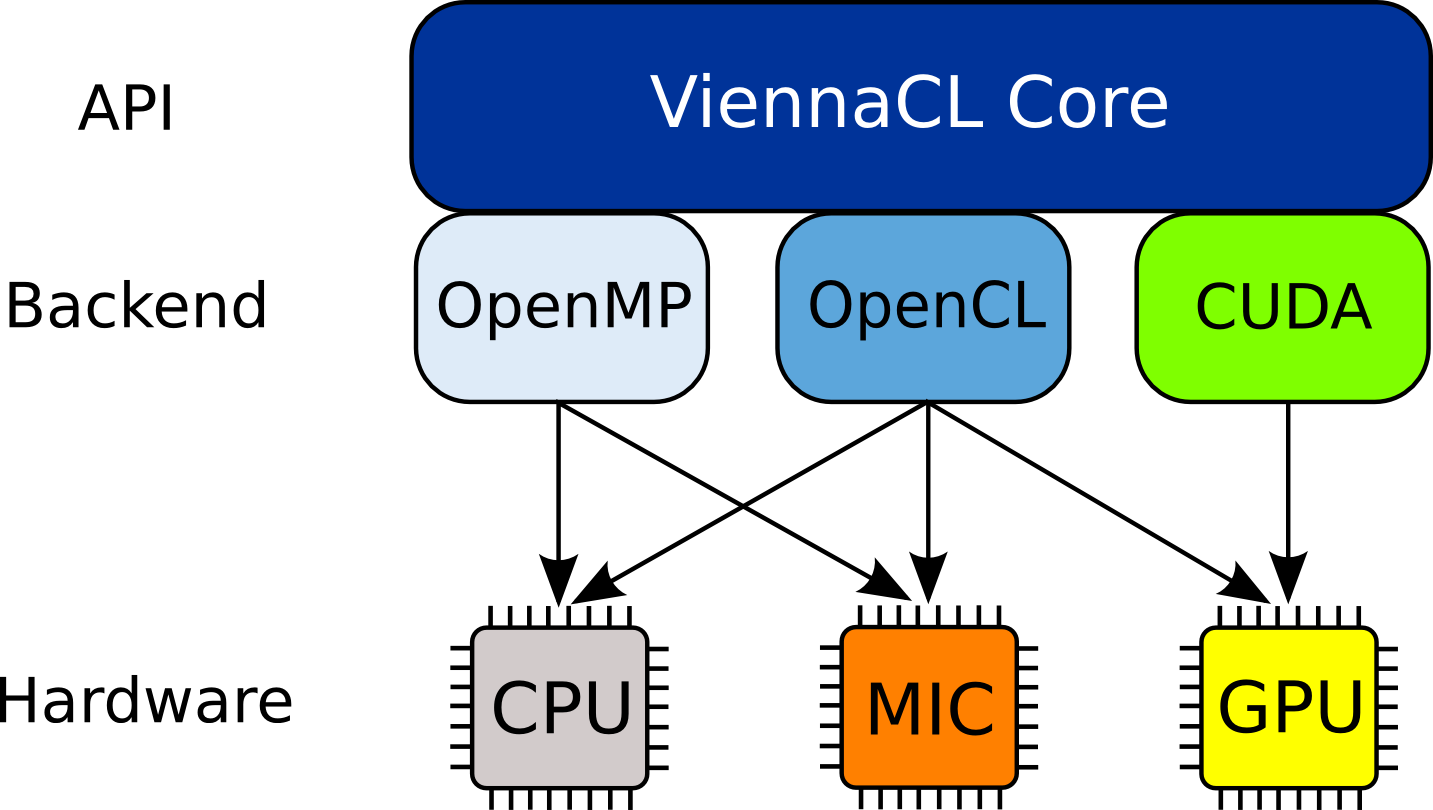
\includegraphics[width=0.6\textwidth]{figs/ViennaCL-arch.png}
  \end{center}
 \end{block}

\end{frame}



\begin{frame}[fragile]
\frametitle{Backends}

\begin{block}{Memory buffer switching at runtime}
\begin{lstlisting}
#define VIENNACL_WITH_OPENCL
#define VIENNACL_WITH_OPENMP

viennacl::vector<float> v1, v2;

switch_memory_domain(v1, MAIN_MEMORY);
switch_memory_domain(v2, MAIN_MEMORY);

v1 += v2; \\ working on CPU with OpenMP

switch_memory_domain(v1, OPENCL_MEMORY);
switch_memory_domain(v2, OPENCL_MEMORY);

v1 += v2; \\ working on GPU with OpenCL
\end{lstlisting}
\end{block}

\end{frame}








\begin{frame}{OpenCL kernel management}

\begin{block}{Best kernel implementations depend on target hardware}
  \begin{itemize}
    \item NVIDIA, AMD, Intel
  \end{itemize}
\end{block}

\begin{block}{Best work group size depends on target hardware}
  \vspace{0.3cm}
  \begin{tabular}{l|llll|llll}
    \multicolumn{5}{c}{ \hspace{0.6cm} NVIDIA} & \multicolumn{4}{c}{AMD} \\
    & 32  & 64  & 128 & 256 & 32 & 64 & 128 & 256 \\
    \hline
    64  & 191 & 151 & 174 & 193 & 324 & 262 & 256 & 249 \\
    128 & 194 & 177 & \textbf{195} & 214 & 357 & 290 & \textbf{272} & \textbf{247} \\
    256 & 161 & 164 & 195 & 214 & 307 & 264 & 256 & 248 \\
    512 & \textbf{145} & 157 & 198 & 211 & 282 & 255 & 258 & 253 \\
  \end{tabular}
  \vspace{0.3cm}
  \\Execution times for sparse matrix-vector product in milliseconds
\end{block}

\end{frame}



\begin{frame}[fragile]
\frametitle{OpenCL kernel management}

\begin{block}{Kernel parameter tuning}
  \begin{itemize}
    \item Default number of work groups = 128
    \item Default number of work items per work group = 128
    \item Automatic tuning environment $\Rightarrow$ XML file
  \end{itemize}
\end{block}

\begin{block}{How to use kernel parameters}
\begin{lstlisting}
using namespace viennacl;
using viennacl::io;

read_kernel_parameters< vector<float> >
    ("float_vector_parameters.xml");
read_kernel_parameters< matrix<float> >
    ("float_matrix_parameters.xml");
read_kernel_parameters< compressed_matrix<float> >
    ("float_sparse_parameters.xml");
\end{lstlisting}
\end{block}

\end{frame}



\begin{frame}{OpenCL kernel management}

\begin{block}{ViennaCL expression template don't cover all operations}
  \begin{itemize}
    \item Sample operation: $\mathbf{x} = \mathbf{A} \times \bigl[ (\mathbf{y} \cdot (\mathbf{y}+\mathbf{z}))\mathbf{y} + \mathbf{z} \bigr]$
  \end{itemize}
\end{block}

\begin{block}{Automated kernel generation}
  \begin{itemize}
    \item Supported since ViennaCL 1.3.0
    \item Experimental support
  \end{itemize}
\end{block}

\begin{block}{Symbolic variables}
  \begin{itemize}
    \item Operation is defined with C++ symbolic variables
    \item Custom kernel object is generated
  \end{itemize}
\end{block}

\end{frame}



\begin{frame}[fragile]
\frametitle{OpenCL kernel management}

\begin{block}{Automated kernel generation}
  \begin{itemize}
    \item Sample operation: $\mathbf{x} = \mathbf{A} \times \bigl[ (\mathbf{y} \cdot (\mathbf{y}+\mathbf{z}))\mathbf{y} + \mathbf{z} \bigr]$
  \end{itemize}
  \begin{lstlisting}
// Instantiation of the symbolic variables
symbolic_vector<NumericType, 0> sX;
symbolic_matrix<NumericType, 1> sA;
symbolic_vector<NumericType, 2> sY;
symbolic_vector<NumericType, 3> sZ;

//Creation of the custom operation
custom_operation my_op(
    sX = prod(sA, inner_prod(sY, sY+sZ) * sY + sZ),
    "operation_name" );
  \end{lstlisting}
\end{block}

\end{frame}



\begin{frame}[fragile]
\frametitle{OpenCL kernel management}

\begin{block}{Automated kernel execution}
  \begin{lstlisting}
viennacl::vector<NumericType> x, y, z;
viennacl::matrix<NumericType> A;
  
// fill data here
  
//Execution of the custom operation
viennacl::ocl::enqueue(my_op(x,A,y,z));
  \end{lstlisting}
\end{block}

\end{frame}





\begin{frame}[fragile]
\frametitle{Extending ViennaCL}

\begin{block}{Not Everything Covered by ViennaCL}
 \begin{itemize}
  \item Complicated vector expressions in a single compute kernel
 \end{itemize}
\end{block}

\begin{block}{Direct OpenCL Kernel Handling is a Pain}
  \begin{lstlisting}
const char * my_kernel_sources = 
"__kernel void element_prod(\n"
"          __global const float * vec1,\n"
"          __global const float * vec2, \n"
"          __global float * result,\n"
"          unsigned int size) \n"
"{ \n"
"  for (unsigned int i = get_global_id(0);  \n"
"                    i < size;  \n"
"                    i += get_global_size(0))\n"
"    result[i] = vec1[i] * vec2[i];\n"
"};\n";
  \end{lstlisting}
\end{block}

\end{frame}


\begin{frame}[fragile]
\frametitle{Extending ViennaCL}

\begin{block}{The OpenCL Way (error checks and casts omitted)}
  { \lstset{ basicstyle=\scriptsize\ttfamily } \begin{lstlisting}
size_t source_len = std::string(my_compute_program).length();
cl_program my_prog = clCreateProgramWithSource(my_context, 1, 
                         &my_kernel_sources, &source_len, &err);
err = clBuildProgram(my_prog, 0, NULL, NULL, NULL, NULL);

const char * kernel_name = "element_prod";
cl_kernel my_kernel = clCreateKernel(my_prog, kernel_name, &err);

err = clSetKernelArg(my_kernel, 0, sizeof(cl_mem), &mem_vec1);
err = clSetKernelArg(my_kernel, 1, sizeof(cl_mem), &mem_vec2);
err = clSetKernelArg(my_kernel, 2, sizeof(cl_mem), &mem_result);
err = clSetKernelArg(my_kernel, 3, sizeof(unsigned int), &vsize);
err = clEnqueueNDRangeKernel(queues[0], my_kernel, 1, NULL, 
                       &global_size, &local_size, 0, NULL, NULL);
  \end{lstlisting} }
\end{block}

 \begin{block}{Issues}
  \begin{itemize}
   \item Access \texttt{my\_kernel} at some other location in an application?
   \item What to do with \texttt{my\_prog}?
  \end{itemize}
 \end{block}

  

\end{frame}



\begin{frame}[fragile]
\frametitle{Extending ViennaCL}

\begin{block}{The ViennaCL Way (namespaces omitted)}
  {\black \begin{lstlisting}
program & my_prog = 
  current_context().add_program(my_kernel_sources, 
                                "my_program");
kernel & my_kernel = my_prog.add_kernel("element_prod");
enqueue(my_kernel(vec1, vec2, result, vec1.size()) );
  \end{lstlisting} }
\end{block}

\begin{block}{At any other Location within the Application}
  {\black \begin{lstlisting}
kernel & my_kernel = get_kernel(
    "my_program", "element_prod");
viennacl::ocl::enqueue(
    my_kernel(vec1, vec2, result, vec1.size()) );
  \end{lstlisting} }
\end{block}

  \begin{block}{Allows for Adding Missing Functionality Easily}
    \begin{itemize}
     \item A bit of OpenCL knowledge required
    \end{itemize}
  \end{block}

\end{frame}



\begin{frame}[fragile]
\frametitle{Extending ViennaCL}

\begin{block}{Integrate ViennaCL into User-Environment}
 \begin{itemize}
  \item User-provided context, queue and device
 \end{itemize}
\end{block}

  \begin{lstlisting}
cl_context my_context = ...; //a context
cl_device_id my_device = ...; //a device in my_context
cl_command_queue my_queue = ...; //a queue for my_device
// supply existing context 'my_context' with one device 
// and one queue to ViennaCL using id '0':
viennacl::ocl::setup_context(0, my_context, my_device, my_queue);
  \end{lstlisting}

\begin{block}{Wrapping Memory Buffers}
  \begin{lstlisting}
   cl_mem my_memory = ...;
   viennacl::vector<float> my_vec(my_memory, 10);
  \end{lstlisting}
 \begin{itemize}
  \item Use ViennaCL operations as usual
 \end{itemize}

\end{block}

\end{frame}



\begin{frame}{ViennaCL and OpenGL}

\begin{block}{ViennaCL and OpenGL}
  \begin{itemize}
    \item Since OpenCL 1.1: OpenGL interoperability
    \item With own OpenCL context: easy task
  \end{itemize}
\end{block}

\begin{block}{Workflow}
  \begin{itemize}
    \item Setup OpenGL and OpenCL
    \item Create OpenGL buffer and OpenCL memory object
    \item Pass OpenCL memory object to ViennaCL
    \item Do ViennaCL magic
    \item Use data in OpenGL
  \end{itemize}
\end{block}

\end{frame}



\begin{frame}[fragile]
\frametitle{ViennaCL and OpenGL}

\begin{block}{Setup OpenGL context (simple glut-glew magic)}
  \begin{lstlisting}
glutInit(&argc, argv);
    
glutInitDisplayMode(...);
glutInitWindowPosition(100,100);
glutInitWindowSize(1600,800);
glutCreateWindow("CL - GL");
    
glewInit();
  \end{lstlisting}
\end{block}

\end{frame}



\begin{frame}[fragile]
\frametitle{ViennaCL and OpenGL}

\begin{block}{Setup OpenCL context with OpenGL interoperability support}
  \begin{lstlisting}
cl_context_properties properties[] = {
    CL_GL_CONTEXT_KHR, (cl_context_properties)
        glXGetCurrentContext(),
    CL_GLX_DISPLAY_KHR, (cl_context_properties)
        glXGetCurrentDisplay(),
    CL_CONTEXT_PLATFORM, (cl_context_properties)
        viennacl::ocl::get_platforms()[0].id(),
    0};
    
cl_device_id my_device =
    viennacl::ocl::current_device().id();
        
cl_context my_context = clCreateContext(properties, 1,
    &my_device, NULL, NULL, &err);
cl_command_queue my_queue = clCreateCommandQueue(
    my_context, my_device, 0, &err );
  \end{lstlisting}
\end{block}

\end{frame}


\begin{frame}[fragile]
\frametitle{ViennaCL and OpenGL}

\begin{block}{Setup OpenCL context with OpenGL interoperability support}
  \begin{lstlisting}
cl_context_properties properties[] = {
    |\color{red}CL\_GL\_CONTEXT\_KHR, (cl\_context\_properties)|
        |\color{red}glXGetCurrentContext()|,
    |\color{red}CL\_GLX\_DISPLAY\_KHR, (cl\_context\_properties)|
        |\color{red}glXGetCurrentDisplay()|,
    |\color{red}CL\_CONTEXT\_PLATFORM, (cl\_context\_properties)|
        |\color{red}viennacl::ocl::get\_platforms()[0].id()|,
    0};
    
cl_device_id my_device =
    viennacl::ocl::current_device().id();
        
cl_context my_context = clCreateContext(properties, 1,
    &my_device, NULL, NULL, &err);
cl_command_queue my_queue = clCreateCommandQueue(
    my_context, my_device, 0, &err );
  \end{lstlisting}
\end{block}

\end{frame}



\begin{frame}[fragile]
\frametitle{ViennaCL and OpenGL}

\begin{block}{Setting up ViennaCL for our context}
  \begin{lstlisting}
viennacl::ocl::setup_context( 
    0,          // the ViennaCL context ID
    my_context, // our context with OpenGL interoperability
    my_device,  // the device we are working on
    my_queue ); // the command queue for our context
    
// tell ViennaCL that we want to use our context
viennacl::ocl::switch_context( 0 );
  \end{lstlisting}
\end{block}

\end{frame}




\begin{frame}[fragile]
\frametitle{ViennaCL and OpenGL}

\begin{block}{Create OpenGL buffer and OpenCL memory object}
  \begin{lstlisting}
glGenBuffers(1, &gl_buffer);
glBindBuffer( GL_PIXEL_UNPACK_BUFFER, gl_buffer );
glBufferData( GL_PIXEL_UNPACK_BUFFER, size, NULL, GL_DYNAMIC_COPY );

cl_mem cl_buffer = clCreateFromGLBuffer(my_context, CL_MEM_READ_WRITE, gl_buffer, &err);
  \end{lstlisting}
\end{block}

\end{frame}



\begin{frame}[fragile]
\frametitle{ViennaCL and OpenGL}

\begin{block}{ViennaCL magic}
  \begin{lstlisting}
// Create viennacl vector from OpenCL memory
viennacl::vector<float> my_vec(cl_buffer, size);

// Acquire memory object for write read/write operation
clEnqueueAcquireGLObjects(my_queue, 1, &cl_buffer,
    0, NULL, NULL);

// copy CPU data to ViennaCL
viennacl::copy( tmp_vec, my_vec );
// doing some stuff
my_vec *= 0.5f;

// Release memory object
clEnqueueReleaseGLObjects(my_queue, 1, &cl_buffer,
    0, NULL, NULL);
  \end{lstlisting}
\end{block}

\end{frame}



\begin{frame}[fragile]
\frametitle{ViennaCL and OpenGL}

\begin{block}{ViennaCL magic}
  \begin{lstlisting}
// Create viennacl vector from OpenCL memory
viennacl::vector<float> my_vec(cl_buffer, size);

// Acquire memory object for write read/write operation
|\color{red}clEnqueueAcquireGLObjects(my\_queue, 1, \&cl\_buffer,|
    |\color{red}0, NULL, NULL);|

// copy CPU data to ViennaCL
viennacl::copy( tmp_vec, my_vec );
// doing some stuff
my_vec *= 0.5f;

// Release memory object
|\color{red}clEnqueueReleaseGLObjects(my\_queue, 1, \&cl\_buffer,|
    |\color{red}0, NULL, NULL);|
  \end{lstlisting}
\end{block}

\end{frame}



\begin{frame}{ViennaCL and OpenGL}

Lets take a look at this example

\end{frame}



\begin{frame}{Summary}
\begin{block}{What have we learned?}
  \begin{itemize}
   \item ViennaCL has different backends
   \item How to enable and use backends
   \item OpenCL management in ViennaCL
   \item How to use an own OpenCL kernel with ViennaCL
   \item How to provide own OpenCL contexts
   \item ViennaCL works with OpenGL!
   \item How to use ViennaCL to work with OpenGL
  \end{itemize}
\end{block}
\end{frame}


% \begin{frame}{Summary}
% \TODO{Achievement unlocked: ViennaCL god}
% \end{frame}







% Conclustion




\begin{frame}{Acknowledgements}

 \begin{minipage}{0.5\textwidth}
  \begin{block}{Contributors}
    \begin{itemize}
     \item Thomas Bertani
     \item Evan Bollig
     \item Philipp Grabenweger
     \item Volodymyr Kysenko
     \item Nikolay Lukash
     \item G\"unther Mader
     \item Vittorio Patriarca
     \item Florian Rudolf
     \item Astrid Rupp
     \item \textbf{Karl Rupp}
     \item Philippe Tillet
     \item Markus Wagner
     \item Josef Weinbub
     \item Michael Wild
    \end{itemize}
  \end{block}
 \end{minipage}
 \begin{minipage}{0.4\textwidth}
  
\includegraphics[width=0.65\textwidth]{figs/gsoc2011.png}
  \vspace*{0.2cm} \\
  
\includegraphics[width=0.65\textwidth]{figs/gsoc2012.png}
  \vspace*{0.2cm} \\
  
\includegraphics[width=0.65\textwidth]{figs/nvidia_logo_black.png}
  \vspace*{0.2cm} \\
  
\includegraphics[width=0.65\textwidth]{figs/amd-logo.png}
 \end{minipage}

\end{frame}



\begin{frame}{Summary}
 
 \begin{block}{High-Level C++ Approach of ViennaCL}
  \begin{itemize}
   \item Convenience of single-threaded high-level libraries (Boost.uBLAS)
   \item Header-only library for simple integration into existing code
   \item MIT (X11) license
   \item \centering http://viennacl.sourceforge.net/
  \end{itemize}
 \end{block}

 \begin{block}{Selected Features}
  \begin{itemize}
   \item Backends: OpenMP, OpenCL, CUDA
   \item Iterative Solvers: CG, BiCGStab, GMRES
   \item Preconditioners: AMG, SPAI, ILU, Jacobi
   \item BLAS: Levels 1-3
   \item 
  \end{itemize}
 \end{block}

\end{frame}


%%
%%
%%  Part 1: Algorithmic Aspects
%%
%%

%\input{algorithmic}


%%
%%
%%  Part 2: Software Aspects
%%
%%

%\input{software}


%%
%%
%%  Part 3: Current and Future Topics
%%
%%

%\input{future}




\end{document}

